\documentclass[times, utf8, diplomski, numeric]{fer}
\usepackage{booktabs}
\usepackage{nameref}
\usepackage{listings}
\usepackage{bchart}
\usepackage{adjustbox}
\usepackage{float}

\usepackage{xcolor}

\colorlet{punct}{red!60!black}
\definecolor{background}{HTML}{EEEEEE}
\definecolor{delim}{RGB}{20,105,176}
\colorlet{numb}{magenta!60!black}

\lstdefinelanguage{json}{
    basicstyle=\normalfont\ttfamily,
    numbers=left,
    numberstyle=\scriptsize,
    stepnumber=1,
    numbersep=8pt,
    showstringspaces=false,
    breaklines=true,
    frame=lines,
    backgroundcolor=\color{background},
    literate=
     *{0}{{{\color{numb}0}}}{1}
      {1}{{{\color{numb}1}}}{1}
      {2}{{{\color{numb}2}}}{1}
      {3}{{{\color{numb}3}}}{1}
      {4}{{{\color{numb}4}}}{1}
      {5}{{{\color{numb}5}}}{1}
      {6}{{{\color{numb}6}}}{1}
      {7}{{{\color{numb}7}}}{1}
      {8}{{{\color{numb}8}}}{1}
      {9}{{{\color{numb}9}}}{1}
      {:}{{{\color{punct}{:}}}}{1}
      {,}{{{\color{punct}{,}}}}{1}
      {\{}{{{\color{delim}{\{}}}}{1}
      {\}}{{{\color{delim}{\}}}}}{1}
      {[}{{{\color{delim}{[}}}}{1}
      {]}{{{\color{delim}{]}}}}{1},
}

\lstset{language=Python, tabsize=4}

\newcommand{\norm}[1]{\left\lVert#1\right\rVert}
\newcommand{\abs}[1]{\left\lvert#1\right\rvert}

\begin{document}

% Navedite broj rada.
\thesisnumber{1147}

% Navedite naslov rada.
\title{Semantička segmentacija prirodnih scena dubokim neuronskim mrežama}

% Navedite vaše ime i prezime.
\author{Ivan Borko}

\maketitle

% Ispis stranice s napomenom o umetanju izvornika rada. Uklonite naredbu \izvornik ako želite izbaciti tu stranicu.
\izvornik

% Dodavanje zahvale ili prazne stranice. Ako ne želite dodati zahvalu, naredbu ostavite radi prazne stranice.
\zahvala{}

\tableofcontents

\chapter{Uvod}

Razumijevanje scene osnovni je problem mnogih segmenata računalnog vida. Jedan od načina na koji se može ostvariti razumijevanje scene je semantička segmentacija, odnosno proces pridjeljivanja semantičkih oznaka dijelovima slike. Primjeri oznaka su: nebo, more, livada, stablo, automobil, osoba, zgrada. Scena je obično predstavljena digitalnom fotografijom pa onda govorimo o pridjeljivanju oznaka svakom pikselu.

Razumijevanje scene bitan je dio mnogih autonomnih robotiziranih sustava koji čine interakcije s okolinom.
Primjer su autonomni automobili koji su u zadnje vrijeme postigli veliki razvojni napredak pa često svjedočimo reportažama o vožnjama ili pak testovima novih prototipova. Takvi automobili koriste sustave za razumijevanje scene kako bi pratili cestu kojom voze, pratili druge sudionike u prometu i mogli izbjeći potencijalne nesreće.

Ovaj rad opisuje sustav za semantičku segmentaciju koji koristi već segmentirane scene za "učenje" svojih parametara. Arhitektura sustava se temelji na dubokim neuronskim mrežama, konkretno konvolucijskim neuronskim mrežama. Sustavi temeljeni na konvolucijskim mrežama postižu najbolje rezultate \engl{state-of-the-art} u mnogim zadacima računalnog vida poput klasifikacije (\cite{krizhevsky_imagenet}, \cite{googlenet}, \cite{vgg_net}, \cite{overfeat}), detekcije objekata (\cite{girshick2014rcnn}), fine kategorizacije \engl{fine grained categorization}(\cite{zhang14finegrained}) i semantičke segmentacije (\cite{farabet_pami}, \cite{long_shelhamer}, \cite{ChenPKMY14}).

Do prije četiri godine godine konvolucijske mreže nisu bile glavni alat za semantičku segmentaciju. Tada su se uglavnom koristile razne metode temeljene na grafovima i grupiranju piksela u skupine. U takvim postupcima često se za svaku regiju koja predstavlja okolinu piksela računaju HOG \engl{histogram of gradients} ili SIFT \engl{scale invariant feature transform} opisnici \cite{Lowe:1999}. Ti opisnici predstavljaju značajku te regije i ulaze u klasifikator koji ih zatim klasificira i grupira.
Kod korištenja klasifikatora temeljenih na stablima odluka opet se učenjem parametara minimizira funkcija gubitka. Parametri stabla su parametri podjele podataka u svakom čvoru \engl{decision stump parameters} i oni se kod stabala uče uzorkovanjem, budući da je podjela podataka nederivabilna funkcija.

U drugom su poglavlju opisane neuronske mreže: od njihove prve ideje, kroz razvoj perceptrona i logističke regresije sve do današnjih dubokih neuronskih mreža, posebice konvolucijskih neuronskih mreža. U trećem poglavlju opisane su metode učenja neuronskih mreža: metode gradijentnog spusta i vrste regularizacija. Četvrto poglavlje opisuje pojam semantičke segmentacija i korištene skupove podataka. U petom se poglavlju opisuju detalji programske implementacije konvolucijske neuronske mreže iz ovog rad, a šestom su opisani rezultati koje je implementirana mreža postigla. U sedmom je poglavlju dan zaključak rada.

\chapter{Neuronske mreže}

Umjetne neuronske mreže \engl{artificial neural networks} ili skraćeno neuronske mreže su paradigma koja opisuje procesiranje informacija inspirirano načinom na koji ljudski mozak (promatran samo kao skup neurona) procesira informacije, odnosno električne impulse. Glavna odlika neuronske mreže je procesiranje informacija jednostavnim elementima (neuronima) koji omogućavaju visoku razinu paralelizma. Ti jednostavni elementi su međusobno povezani velikim brojem veza (u biološkom sustavu te veze su sinapse). Učenje neuronskog biološkog sustava podrazumijeva podešavanje sinapsi, a slično tome se podešavaju parametri u umjetnoj neuronskoj mreži.

Osnovni element umjetne neuronske mreže je umjetni neuron. Prvi umjetni neuron, nazvan perceptron, razvio je Frank Rosenblatt 1950-ih inspiriran ranijim radom \cite{mcculloch43a}  Warrena  McCullocha i Waltera Pittsa iz 1943. o njihovom viđenju umjetnog neurona. Taj početni entuzijazam nije predugo trajao jer Minsky i Papert 1969. godine objavljuju knjigu \cite{minsky69perceptrons} u kojoj navode mane neuronskih mreža i daju pesimističan pogled na neuronske mreže. Tada većina znanstenika prestaje s istraživanjima na tome polju i razvoj ostaje na par znanstvenika koji su trebali dokazati mogućnosti neuronskih mreža.

\begin{figure}[htb]
\centering
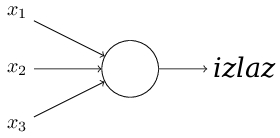
\includegraphics[width=220px]{imgs/percep.png}
\caption{Primjer perceptrona s 3 ulaza}
\label{fig:percep}
\end{figure}

Slika \ref{fig:percep} prikazuje primjer perceptrona koji ima 3 ulaza, $x_1, x_2, x_3$. Općenito, broj ulaza je proizvoljan. Rosenblatt je predstavio pravilo kako se računa izlaz iz neurona: postoje težine $w_1, w_2, ...$, realni brojevi koji predstavljaju značaj pripadajućih ulaza. Izlaz neurona se određuje prema tome je li suma $\sum_{j} w_j \cdot x_j$ veća ili manje od neke fiksne vrijednost. Matematički se to može zapisati kao:
\begin{equation}
izlaz =
\left\{
	\begin{array}{ll}
		0  & \mbox{ako } \sum_j w_j \cdot x_j \leq prag \\
		1  & \mbox{ako } \sum_j w_j \cdot x_j >  prag
	\end{array}
\right.
\end{equation}

Učenje takvog modela se zapravo svodi na podešavanje težina $w_j$ i praga, čime se postižu različite vrijednosti izlaza.

Današnji umjetni neuron koji se koristi u neuronskim mrežama se malo razlikuje od originalne ideje perceptrona po tome što ne koristi step funkciju na izlazu, već neku funckciju iz porodice sigmoidalnih funkcija (neki autori takav neuron nazivaju logistički neuron ili logistički perceptron).

No, nije samo rad Minskog i Paperta kočio razvoj neuronskih mreža: računalna snaga je tada bila veliko ograničenje. Zato su se proučavali tek jednostavni modeli, koji nisu imali dovoljnu moć. Prava moć dolazi tek kada se više perceptrona spoji zajedno kroz više slojeva (vidi poglavlje \ref{chap:viseslojni_perceptron}). Tijekom 80-ih godina dolazi do razvoja računalnog paralelizma i povećanja računalne snage čime rastu mogućnosti za treniranje i evaluacije kompleksnijih neuronskih mreža.

Značajan napredak postigao je i Werbos 1975. godine kada je u svojem radu \cite{Werbos:74} primjenio algoritam unazadne propagacije \engl{backpropagation} za učenje neuronskih mreža (vidi poglavlje Backgropagation).
Često se taj trenutak naziva i renesansom neuronskim mreža jer opisani postupak omogućava lako treniranje neuronskih mreža neovisno o njihovoj složenosti i arhitekturi.

Za to vrijeme snažno su se razvijali drugi algoritmi strojnog učenja. Stroj s potpornim vektorima \engl{support vector machine}, ili kraće SVM, tako postaje moćniji i zastupljeniji klasifikator od neuronskih mreža. Tek zadnjih 10-ak godina duboke neuronske mreža polako preuzimaju primat SVM-a zbog dolaska GPGPU \engl{general purpose graphics processsing unit} jedinica koje su sposobne izvršavati velike količine paraleliziranih matričnih operacija potrebnih za treniranje dubokih mreža.

\section{Klasifikacija i regresija}
Dva temeljna problema prediktivnih sustava su klasifikacija i regresija.
Klasifikacija je razvrstavanje ulaznih podatka u jedan od $K$ razreda. Ako je $K = 2$ onda govorimo o binarnoj klasifikaciji. Kod neuronskih mreža se to može ostvariti postavljanjem step funkcije na na kraj zadnjeg neurona čime izlaz postaje 0 ili 1.
Ako je $K > 2$ onda pak govorimo o višeklasnoj \engl{multiclass} klasifikaciji. Postoji još i verzija klasifikacije s više klasa koja svakom primjeru pridjeljuje podskup dogovorenog skupa klasa \engl{multi-label classification}, odnosno jedan primjer može spadati u više klasa.
Za razliku od klasifikacije, regresija daje realni broj kao izlaz. Cilj je da realni izlaz bude čim sličniji traženom izrazu.

\section{Nadzirano i nenadzirano učenje}
Dva su glavna pristupa učenju prediktivnih modela koja vrijede i za neuronske mreže: nadzirano i nenadzirano učenje. Tijekom nadziranog učenja mreži prezentiramo par podataka $(x, y), x \in X, y \in Y$, gdje je X skup svih ulaza u mrežu, a Y skup pripadnih izlaznih (traženih) vrijednosti.
Cilj je pronaći funkciju $f: X \to Y$, koja aproksimira preslikavanje implicirano u podacima za učenje.

Parametri modela se optimiraju tako da se smanjuje zadana funkcija troška \engl{cost function}. Funkcija troška može biti srednja kvadratna pogreška između traženih i dobivenih vrijednosti na izlazu (većinom korištena za regresijske probleme),
\begin{equation}
	\mathcal{L} = (y_t - y_p)^2
\end{equation}
ili pak pogreška unakrsne entropije (koristi se za binarnu klasifikaciju)
\begin{equation}
	\mathcal{L} = -(y_t \log(y_p) + (1 - y_t) \log(1 - y_p))
\end{equation}

gdje je $y_t$ je tražena vrijednost na izlazu, a $y_p$ je dobivena (predviđena) vrijednost.

Tijekom nenadziranog učenja nema izlaznog skupa podataka, samo ulazni skup $X$. Dana je i funkcija troška koja se optimira.
Cilj može biti kompresija ulaznog višedimenzionalnog vektora u manje dimenzionalan pa je funkcija troška zapravo kvadratna pogrška rekonstrukcije. Ili se pak traži grupiranje podataka u $K$ grupa (primjer je \textit{K-means} algoritam\cite{Hartigan-1979}) koje se isto tako može formulirati kao pronalaženje kodova (centara) koji minimiziraju kvadratnu pogrešku.


\section{Logistička regresija}
\label{chap:logisticka_regresija}

Originalni perceptron se razvijao kroz povijest i njegova verzija koja se trenutno koristi u neuronskim mrežama izgleda malo drugačije. Ulazi više ne moraju biti binarne vrijednosti, već to mogu biti realne vrijednosti, a funkcija na izlazu je sigmoid (logistička funkcija), definirana formulom:
\begin{equation}
f(x) = \frac{1}{1+e^{-x}}
\end{equation}

Takav se model naziva logistička regresija. Logistička regresija je jedan od osnovnih klasifikacijskih modela, iako joj ime govori da je to regresijski model, što ona nije.
Logistička regresija je probabilistički klasifikator jer njezin izlaz predstavlja vjerojatnost da je primjer u određenom razredu.\cite{strojno_snajder}
Ona je i linearni klasifikator jer je decizijska granica linearna.
Kod jednostavne (dvoklasne) klasifikacije parametri logističke regresije su vektor težina $\boldsymbol{w}$ i pomak $\boldsymbol{b}$. Vektor težina predstavlja težine svakog neurona, odnosno element vektora težina na poziciji $i$ se množi s podatakom na $i$-tom ulazu.
\begin{equation}
  \sum_i w_i \cdot x_i + b = \boldsymbol{w} \bullet \boldsymbol{x} + b
\end{equation}

Za višeklasnu klasifikaciju postoji multinomijalna regresija kojoj su parametri matrica težina $W$ i vektor pomaka $\boldsymbol{b}$, a kao aktivacijska funkcija se koristi \textit{softmax} funkcija:
\begin{equation}
  \mathrm{softmax} \left( \boldsymbol{z} \right)_j = \frac{e^{z_j}}{\sum_{k=1}^{K} e^{z_k}} \quad \mathrm{za} \  j = 1, ..., K
\end{equation}
gdje je $\boldsymbol{z}$ je argument funkcije ($K$-dimenzionalni vektor). Vrijednosti funkcije za svaku komponentu $j$ su između 0 i 1. Može se pokazati da su te vrijednosti uvjetne vjerojatnosti komponenata. Iz toga slijedi kako su vjerojatnosti da neki primjer pripada u jednu od $K$ klasa sljedeće:
\begin{equation}
  P \left( y_p = j | \boldsymbol{x} \right) = \frac{e^{\boldsymbol{w}_j \bullet x}}{\sum_{k=1}^{K} e^{\boldsymbol{w}_k \bullet x}} \quad \mathrm{za} \  j = 1, ..., K
\end{equation}
gdje je $y_p$ predviđena vrijednost primjera $\boldsymbol{x}$.

Klasifikacija se vrši tako da se određuje projekcija točaka u n-dimenzionalnom prostoru na normalu hiperravnine koja predstavljaja granicu između razreda uzoraka.

Matematički se to može zapisati kao:
\begin{equation}
P(Y = 1 | \boldsymbol{x}, \boldsymbol{w}, b) = f(\boldsymbol{w} \bullet \boldsymbol{x} + b) = \frac{1}{1+e^{-(\boldsymbol{w} \bullet \boldsymbol{x} + b)}}
\label{eq:sigmoid}
\end{equation}
gdje je $f$ sigmoidalna funkcija, $\bullet$ skalarni produkt vektora, $\boldsymbol{x}$ ulazni vektor, a $Y$ je skup izlaznih vrijednosti (1 znači da pripada nekom razredu).

Odnosno kao
\begin{equation}
P(Y = i | \boldsymbol{x}, W, b) = \mathrm{softmax}(W^T \cdot \boldsymbol{x} + b) = \frac{e^{\boldsymbol{x}^{\top} \bullet \boldsymbol{w_i}}}{ \sum_{k=1}^K  e^{\boldsymbol{x}^{\top} \bullet \boldsymbol{w_k}}}
\label{eq:softmax}
\end{equation}
za višeklasnu klasifikaciju ($i$ je oznaka klase kojoj pripada primjer $\boldsymbol{x}$).

Izlaz modela je tada jednak:
\begin{equation}
h = \arg\max_i P(Y = i|\boldsymbol{x}, W, b)
\label{eq:model_out_arg}
\end{equation}


Učenje modela logističke regresije svodi se na određivanje parametera, odnosno vektora težina $\boldsymbol{w}$ i pomaka b. Određivanje parametara se pak svodi na optimiranje funkcije gubitka. Funkciju gubitka možemo definirati kao negativnu log-izglednost na skupu za učenje:
\begin{equation}
  E \left( h | \mathcal{D} \right) = E \left( \boldsymbol{w} | \mathcal{D} \right) = -\ln \mathcal{L} \left( \boldsymbol{w} | D \right)
\end{equation}
gdje je $E$ funkcija gubitka, $\boldsymbol{w}$ je vektor težina, $\mathcal{D}$ je skup svih primjera za učenje $\{ (x^{(i)}, y_t^{(i)}) \}_{i=1}^{N}$, a $y_p$ je izlaz modela: $y_p(x) = f(\boldsymbol{x} \bullet \boldsymbol{w} + b)$.
Izglednost skupa parametara $\theta$, uz poznate ishode $x$, jednaka je vjerojatnosti promatranih ishoda uz poznate vrijednosti parametara:
\begin{equation}
  \mathcal{L} ( \theta | x ) = P ( x | \theta )
\end{equation}
U tom slučaju je učenje modela zapravo maksimizacija log izglednosti.

U skupu za učenje $\mathcal{D} = \{ (x^{(i)}, y_t^{(i)}) \}_{i=1}^{N}$, oznaka $y^{(i)}$ imati vrijednost 0 ili 1. To znači da je za zadani primjer $x^{(i)}$, oznaka $y_t^{(i)}$ zapravo Bernoullijeva slučajna varijabla, te vrijedi $P(y = 1 | x) = P(y | x)$.
Razdioba Bernoullijeve varijable je:
\begin{equation}
  P \left( y_t | x \right) = y_p^{y_t} (1 - y_p^{1-y_t})
\end{equation}
Funkciju log-izglednosti parametara $\theta$ onda možemo raspisati kao:
\begin{equation}
  \ln \mathcal{L} (\theta | \mathcal{D}) = \ln P(\mathcal{D} | \theta ) = \ln \prod_{i=1}^{N} P(y^{(i)} | x^{(i)}) = \ln \prod_{i=1}^{N} (y_p^{(i)})^{y_t^{(i)}} \left( 1 - (y_p^{(i)})^{1-y_t^{(i)}} \right)
\end{equation}

Izglednost parametara bit će to veća što je točnija klasifikacija, odnosno što je veći h(x). Ili drugačije rečeno, izglednost $P(\mathcal{D} | \theta)$ nam kazuje koliko je vjerojatno da naš model primjere u skupu $\mathcal{D}$ klasificira baš onako kako su označeni, ako parametre modela postavimo u $\theta$.

Sada može funkciju troška definirati kao negativnu log-izglednost:
\begin{equation}
  E \left( \theta | \mathcal{D} \right) = -\ln \mathcal{L} (\theta | \mathcal{D}) = -\sum_{i=1}^{N} \left\{ y_t^{(i)} \ln y_p^{(i)} + \left( 1 - y_t^{(i)} \right) \ln (1 - y_p^{(i)}) \right\}
\end{equation}
gdje je $y_t$ je tražena vrijednost (iz skupa za učenje), a $y_p$ je dobivena (predviđena) vrijednost (izlaz modela).
Ovako definirana funkcija troška se naziva \textbf{pogreška unakrsne entropije} \engl{cross-entropy error}.


\section{Višeslojni perceptron}
\label{chap:viseslojni_perceptron}

Do sada spomenuti modeli i arhitekture modeliraju samo jedan biološki neuron, dok je neuronska mreža skup neurona. Spajanjem više modela neurona u više slojeva (u dubinu) i više neurona u širinu, nastaje neuronska mreža. Najjednostavniji model neuronske mreže naziva se višeslojni perceptron.

Višeslojni perceptron sastoji se od 3 sloja: ulaznog sloja, skrivenog sloja \engl{hidden layer} i izlaznog sloja. Ulazni sloj se sastoji od brojeva koji opisuju neki primjer (vektor značajki nekog primjera), skriveni sloj se sastoji od logističkih neurona i zadnji sloj koji se također sastoji od logističkih neurona (broj izlaznih neurona ovisi o broju razreda u koji se klasificira primjer).

Višeslojni perceptron (slika \ref{fig:mlp}) može se promatrati i kao vrsta logističke regresije kod koje su ulazi transformirani pomoću nelinearne transformacije. Svrha tih transformacija je prebaciti ulazne podatke u prostor više dimenzije gdje oni postaju linearno separabilni (budući da je logistička regresija linearni klasifikator). Transformacije izvodi skriveni sloj i on je dovoljan da MLP postane univerzalni aproksimator. \cite{Hornik-1991}

\begin{figure}[htb]
\centering
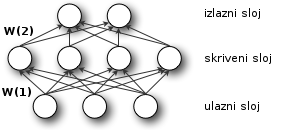
\includegraphics{imgs/mlp.png}
\caption{Višeslojni perceptron}
\label{fig:mlp}
\end{figure}

Izlaz višeslojnog perceptrona je tada:
\begin{equation}
f(\boldsymbol{x}) = G\{\boldsymbol{W}(2) \cdot (s[\boldsymbol{W}(1) \cdot \boldsymbol{x} + \boldsymbol{b}(1))] + \boldsymbol{b}(2)\}
\label{eq:conv}
\end{equation}
$G$ i $s$ su aktivacijske funkcije. Za aktivacijsku funkciju se obično odabire logistička sigmoid funkcija ili $\tanh$. $\tanh$ se odabire jer se višeslojna mreža s njime kao prijenosnom funkcijom brže trenira.
Jednadžba se može protumačiti na način da se izlaz skrivenog sloja $h(\boldsymbol{x}) = s( \boldsymbol{W}(1) * \boldsymbol{x} + \boldsymbol{b} )$ prosljeđuje na ulaz logističke regresije, čime dobijemo višeslojni perceptron.

\section{Duboke neuronske mreže}

Duboke neuronske mreže (ili kraće, DNN) su naziv za neuronske mreže koje sadrže dva ili više skrivena sloja. Takve duboke mreže omogućuju modeliranje komplesnih nelinearnih zavisnosti. Zbog velike količine parametara i same dubine, dugo vremena je treniranje takve mreže bilo problematično, no u zadnjih nekoliko godina, razvile su se metode za njihovo treniranje, ali i same arhitekture koje imaju puno manji broj parametera, a jednaku dubinu i širinu.

Recimo da se želi konstruirati sustav za prepoznavanje lica na slici. Mogli bi koristiti jedan model višeslojnog perceptrona koji bi odgovorio na pitanje postoji li oko u slici, drugi model koji bi pak odgovorio na pitanje postoje li usta na slici, treći model koji bi odgovorio postoji li kosa na slici. Izlaze tih modela bi mogli spojiti na logističku regresiju koja koristi sve izlaze postojećih modela i vraća odgovor postoji li lice na slici. Duboke neuronske mreže mogu zamijeniti takav složeni sustav, jer omogućuju spajanje više slojeva koji se specijaliziraju za različite dubine apstrakcije, a treniranje i korištenje dubokih mreža je jednostavnije od navednog skupa modela i ne zahtijeva ručno smišljanje podjele zadataka.

DNN su obično dizajnirane kao mreže s unaprijednom propagacijom, no posljednja istraživanja pokazuju da je moguće koristiti i povratne neuronske mreže  \engl{recurrent networks} u dubokim arhitekturama (primjer je modeliranje jezika). Jedna specifična verzija dubokih neuronskih mreža su konvolucijske neuronske mreže koje su vrlo često korištene u računalnom vidu (detaljno opisane u poglavlju \ref{chap:konvolucijske_mreze}).

Pokazalo se da je proces treniranja dubokih neuronskih mreža iznimno težak. Algoritmi bazirani na gradijentnim metodama skloni su zapinjanju u sedlastim plohama čime se uvelike usporava konvergencija. Drugi je problem nestajući gradijent \engl{vanishing gradient problem} koji se dešava tijekom unazadne propagacije gradijenata jer se iznos gradijenata smanjuje za red veličine po sloju što znači da se gradijent teško prenosi do prednjih slojeva. Taj se problem rješava korištenjem ne-sigmoidnih aktivacijskih funkcija poput \textit{ReLU} (više u poglavlju \ref{chap:aktivacijske_funkcije}).

Dosta čest argument protiv neuronskih mreža je znao biti da one često zapnu u lokalnim minimumima, ali se pokazalo da su lokalni minimumi u koje mreža ode svi dosta blizu globalnog minimuma. \cite{choromanska14}

Nadalje, iole kompleksnije mreže su vrlo teške za interpretaciju, čak i ako rade dobro, količina parametara je toliko ogromna da je mreža zapravo ''crna kutija'' i nemoguće je analizom ustvrditi zašto dobro rade.

U zadnjih desetak godina slojevitim umjetnim neuronskim mrežama pristupa se na novi način. Radi se s nekoliko tehnika koje imaju nekoliko zajedničkih aspekata.
Kod nekih tehnika (autoenkoderi, ograničeni Boltzmanovi strojevi) slojevi se treniraju jedan po jedan, dok kod drugih (konvolucijske mreže) postoji posebna vrsta slojeva koji imaju smanjen broj parametara i rijetko su povezani čime je smanjen broj operacija po sloju.

Kao zajedničko ime za više tehnika koje na ovaj način pristupaju treniranju umjetne neuronske mreže koristi se termin "duboka neuronska mreža". Duboke neuronske mreže na tipičnim klasifikacijskim problemima postižu rezultate koji su među ponajboljima ikad postignutim.

\subsection{Autoenkoderi}

Autoenkoderi su posebna vrsta umjetnih neuronskih mreža koje se koriste za učenje prikaza informacija u manje memorije (sažimanje), na što se može gledati i kao na metodu smanjivanja značajki ulaznog prostora.
Osnovna ideja autoenkodera je poprilično jednostavna: imamo neuronsku mrežu kojoj ulazni i izlazni sloj imaju jednak broj neurona, u sredinu dodamo još jedan sloj s manjim brojem neurona. Taj srednji sloj, koji je zapravo ''usko grlo'' će naučiti efikasno prikazati ulaze podatke (kodirati ih).

Najjednostavniji model autoenkoderske mreže ima, kao što je već spomenuto, tri sloja (poput MLP-a, poglavlje \ref{chap:viseslojni_perceptron}): ulazni, skriveni i izlazni. Skriveni sloj ima manje neurona od ulaznog, jer se prebacivanjem iz ulaznog u skriveni vrši sažimanje. Postupkom treniranja se nastoji postići da informacija koja dođe na ulazni sloja ($\boldsymbol{x}$) čim sličnija izađe iz izlaznog sloja ($\hat{\boldsymbol{x}}$). Iz toga slijedi da izlazni i ulazni sloj moraju imati jednak broj neurona. Pogreška rekonstrukcije ($\Delta \boldsymbol{x} = \boldsymbol{x} - \hat{\boldsymbol{x}}$) se koristi za podešavanje težina u mreži.
\begin{figure}[htb]
\centering
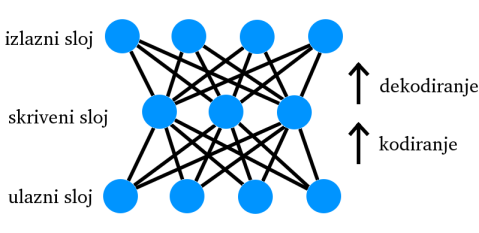
\includegraphics[width=330px]{imgs/autoencoder.png}
\caption{Jednostavni autoenkoder s jednim skrivenim slojem}
\label{fig:autoencoder}
\end{figure}

Hinton je u radu \cite{hinton_autoencoder} prvi upotrijebio autoenkodere kao metodu učenja dubokih neuronskih mreža. Takvim se treniranjem svaki sloj redom uzima kao skriveni sloj autoenkodera i uči. Na kraju se cijela mreža, nastala od tako istreniranih slojeva, spaja i rezultirajuća se mreža fino ugađa primjenom postojećih gradijentnih tehnika.
Treniranjem slojeva pojedinačno poboljšava se pretraga parametarskog prostora mreže: bolje se izbjegavaju lokalni optimumi. Moguće je efikasno trenirati više slojeva koji sadrže veći broj neurona, što omogućuje stvaranje puno kompleksnijih mreža koje se dobro nose s težim zadatcima. Niži slojevi mogu se učiti sa neoznačenim podatcima (polu-nadzirano učenje), čime slojevi uče samo efikasno kodirati informacije na ulazu.
Kod dubokih neuronskih mreža autoenkoderi se koriste samo u situacijama gdje je skup za učenje jako malen i to kao početna faza učenja.

\section{Konvolucijske neuronske mreže}
\label{chap:konvolucijske_mreze}

Duboke neuronske mreže koje sadrže konvolucijske slojeve (pojašnjeni u sljedećem poglavlju) nazivaju se konvolucijskim neuronskim mrežama. Konvolucijske mreže se danas primjenjuju u većini problema računalog vida gdje vrlo često postižu vrhunske rezultate.

\subsection{Konvolucijski sloj}

U zadacima računalnog vida posebno se osjeti rast parametara s dubinom i širinom mreže jer se na ulazu nalaze slike, dimenzija često preko 100x100 piksela (relativno mala slika), što daje 10 000 značajki na ulazu i čini ulazni prostor visoko dimenzionalnim. Uzmimo za primjer mrežu sa 10 000 ulaznih neurona i 1000 skrivenih neurona. Takav prvi sloj ima već 10 milijuna težina, a slaganjem mreže u dubinu se taj broj još povećava, mreža se teško i sporo trenira te je sklona prenaučenosti. Konvolucijski slojevi, u usporedbi sa potpuno povezanim slojevima imaju višestruko manji broj parametara.

Znanstveni radovi temeljeni na vidnom korteksu \engl{visual cortex} mačaka pokazali su da postoji složeni raspored vidnih stanica u oku. Neke od tih stanica osjetljive su na samo malu podregiju vidnog polja nazvanu osjetilno polje \engl{receptive field}. Takve su stanice raspoređene da pokrivaju cijelo vidno polje. Dodatno, identificirana su dva tipa stanica: jednostavne stanice i kompleksne stanice. Jednostavne maksimalno reagiraju na podražajne oblike s izraženim bridovima dok složene imaju veća osjetilna područja i invarijantne su na točnu poziciju podražaja.

Budući da je vizualni korteks trenutno najmoćniji sustav vida, čini se logičnim pokušati emulirati njegovo ponašanje. Mnogi takvi sustavi se mogu pronaći u literaturi: sustav NeoCognitron \cite{neocognitron} je jedan od najranijih pokušaja, a kasnije su uslijedili mnogi drugi \cite{cortex_mehachanism} \cite{gradient_document}.

Važna stvar koju su takvi sustavi pokušali riješiti je i lokalna osjetljivost.
Za područje računalnog vida važno je da se određeni oblici detektiraju neovisno o njihovoj lokaciji na slici. Potpuno povezani sloj ima posebne težine za svaki piksel. To znači da će neki dio mreže moći prepoznati neki oblik samo ako ga vidi na lokacijama na kojima se pojavljivao tijekom učenja, što se želi izbjeći.

Tako se došlo do ideje da bi se mogao koristiti filter koji se pomiče po ulaznom vektoru i na svakoj poziciji pomaka daje određeni izlaz. U slučaju jednodimenzionalnog ulaza jezgra je vektor, u slučaju dvodimenzionalnog ulaza jezgra je matrica, i tako dalje. Takva jezgra ima dimenzije višestruko manje od ulaza (obično 3, 5 ili 7 piksela), čime se rješava i problem velikog broja parametara u dubokim mrežama.

Tako se dolazi do konvolucije, matematičkog pojma definiranog kao učestalo primjenjivanje funkcije na podacima. U ovom konktekstu to znači primjenjivati filter na sliku po svim mogućima pomacima, oponašajući osjetilne stanice u ljudskom oku. Filter predstavlja skup težina povezanih sa prethodnim slojem, gdje je prethodni sloj komadić 2-D ulazne slike, a izlaz je jedan neuron. Takav se filter primjenjuje pomičući kroz cijelu sliku, pri čemu se ''osjetilna polja''' preklapaju, kao što je prikazano na slici \ref{fig:sparse-nn} te nastaje nova 2-D matrica koja se naziva mapa značajki. Jedan konvolucijski sloj sadrži više takvih filtera što ima za posljedicu da nastaje i više mapa značajki.

%(slika http://deeplearning.net/tutorial/_images/sparse_1D_nn.png)
\begin{figure}[htb]
\centering
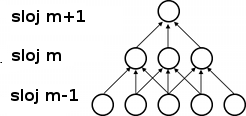
\includegraphics[scale=0.8]{imgs/sparse_1D_nn.png}
\caption{Rijetka povezanost}
\label{fig:sparse-nn}
\end{figure}

Lokalna osjetljivost je u konvolucijskom sloju riješena lokalnom korelacijom neurona, što znači da je neuron $m-1$ sloja povezan samo sa prostorno bliskim neuronima $m$-tog sloja. Na slici \ref{fig:sparse-nn} je primjer lokalnog povezivanja širine 3 neurona za jednodimenzijski ulaz.
Neka je $m-1$ sloj ulazni sloj. Tada je vidno polje neurona u sloju m široko 3 s obzirom na ulaz. Neuroni u sloju $m+1$ su isto povezani s 3 neurona iz prošlog sloja, ali ako se gledaju s obzirom na ulazni sloj, onda je njihovo vidno polje široko 5 neurona. Arhitektura mreže tako ograničava takve ''filtere'' na lokalni uzorak (budući da ne reagiraju na druge dijelove ulaza). Slaganje više takvih slojeva omogućava da ''filteri'' polako postaju globalni (odnosno prostiru se preko većeg broja ulaznih piksela). Na primjer, neuron u sloju $m+1$ može predstavljati \engl{encode} nelinearnu značajku duljine 5.

\begin{figure}[htb]
\centering
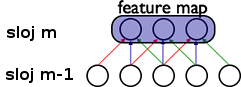
\includegraphics{imgs/conv_1D_nn.png}
\caption{Zajedničke težine}
\label{fig:conv-nn}
\end{figure}

Kod primjene u računalnom vidu, ulazi su uglavnom 2D slike.
Neka ulaz u konvolucijski sloj ima dimezije $x \cdot y \cdot r$, gdje je $x$ širina slike, $y$ visina slike, a $r$ je broj kanala (konkretno za RGB sliku je $r = 3$). Dimenzionalnost konvolucijskog sloja ne ovisi direktno o ulaznom sloju, već samo o broju kanala i iznosi $d \cdot d \cdot r \cdot k$, gdje je $d$ širina odnosno visina filtera za konvoluciju, $r$ je broj kanala prethodnog sloja, $k$ je broj mapa značajki trenutnog sloja (ekvivalent broju kanala na ulazu). Primjer takvog sloja ima filter dimenzija $7 \cdot 7$ i 20 mapa značajki što daje $7 \cdot 7 \cdot 3 \cdot 20 = 2940$ težina, što je značajno manje od milijuna spomenutih na početku poglavlja. Naravno, broj mapa značajki se zna penjati i do nekoliko stotina, no broj težina je i u tom slučaju smanjen naspram potpuno povezanog skrivenog sloja.

Mapa značajki, odnosno izlaz konvolucijskog sloja, se dobije ponavljanim apliciranjem funkcije po podregiji slike, ili drugim rječima, konvolucijom ulazne slike s linearnim filterom, dodajući pristranost sloja $b$ i primjenjujući aktivacijsku funkciju. Ako označimo k-tu mapu značajki nekog sloja kao $h^k$, čiji su filteri određeni težinama $W^k$ i pristranošču $b_k$, onda izlaz takve mape značajki možemo zapisati kao:
\begin{equation}
  h_{ij}^k = f \left( \left( \boldsymbol{W}^k * \boldsymbol{x} \right)_{ij} + \boldsymbol{b}_k \right)
\end{equation}
gdje su $ij$ indeksi ulazne ($x$) odnosno izlazne slike (mape značajki).
U praksi se još svaki konvolucijski sloj sastoji od više mapi značajki, $\{ h^{(k)}, k = 0..K \}$


\subsection{Aktivacijske funkcije}
\label{chap:aktivacijske_funkcije}

Aktivacijska funkcija je funkcija koju koristimo nad izlazima sloja neuronske mreže. % TODO mozda nekako bolje?
Kod logističke regresije aktivacijska funkcija je logistička sigmoid funkcija (formula \ref{eq:logisticka_funkcija}, slika \ref{fig:logistic_sigmoid}) zbog koje je izlaz logističke regresije probabilistički. Logistička funkcija je nelinearna, monotono rastuća funkcija čiji se izlaz asimptotski približava nekoj konačnoj vrijednosti (na primjer, broju 1) dok ulaz raste prema $\pm \inf$.

\begin{figure}[htb]
\centering
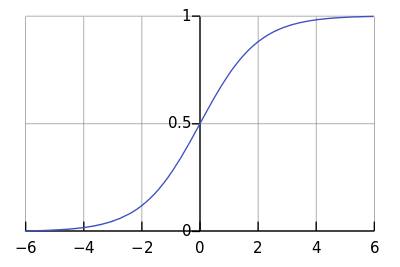
\includegraphics[width=240px]{imgs/logistic_curve.png}
\caption{Logistička sigmoid funkcija}
\label{fig:logistic_sigmoid}
\end{figure}

Osim standardne sigmoid funkcije definirane formulom:
\begin{equation}
f(x) = \frac{1}{1+e^{-x}}
\label{eq:logisticka_funkcija}
\end{equation}
čija je derivacija:
\begin{equation}
\begin{split}
  f' (x) &= \left( \frac{1}{1 + e^{-x}} \right)' = \frac{0 \cdot (1 + e^{-x}) - 1 \cdot (1 + e^{-x})'}{(1 + e^{-x})^2} \\
         &= \frac{-e^{-x} \cdot (-1)}{(1 + e^{-x})^2} = \frac{1}{1 + e^{-x}} \cdot \frac{e^{-x}}{1 + e^{-x}} \\
		 &= \frac{1}{1 + e^{-x}} \cdot \frac{1 - 1 + e^{-x}}{1 + e^{-x}} = \frac{1}{1 + e^{-x}} \cdot \frac{(1 + e^{-x}) - 1}{1 + e^{-x}} \\
		 &= \frac{1}{1 + e^{-x}} \cdot \left[ \frac{1 + e^{-x}}{1 + e^{-x}} + \frac{-1}{1 + e^{-x}} \right] = f(x) \left[ 1 - f(x) \right]
\end{split}
\end{equation}
često se koristi i hiperbolna tangent funkcija $f(x) = \tanh(x)$ (slika \ref{fig:tanh_plot}), isto iz porodice logističkih funkcija.

\begin{equation}
f(x) = \tanh(x) = \frac{\sinh(x)}{\cosh(x)} = \frac{e^{x} - e^{-x}}{e^{x} + e^{-x}} = \frac{e^{2x} - 1}{e^{2x} + 1} = \frac{1 - e^{-2x}}{1 + e^{-2x}}
\label{eq:tanh_def}
\end{equation}
Hiperbolna tangent funkcija se više preferira kao aktivacijska funkcija iz istog razloga zbog kojeg se ulazi normaliziraju: LeCun et al. u radu \cite{lecun-98b} pokazali su da mreže brže konvergiraju ako su ima ulazi normalizirani (translatirani tako da im je srednja vrijednost 0 i standardna deviacija 1). Izlazi jednog sloja su ulaz u drugi iz čega slijedi da bi i izlazi trebali biti u prosjeku oko nule, što se postiže $\tanh$ funkcijom, dok su izlazi sigmoid funkcije pozitivni i centrirani oko 0.5 (ili neke druge pozitivne vrijednosti, ovisno o konkretnom obliku funkcije).

\begin{figure}[htb]
\centering
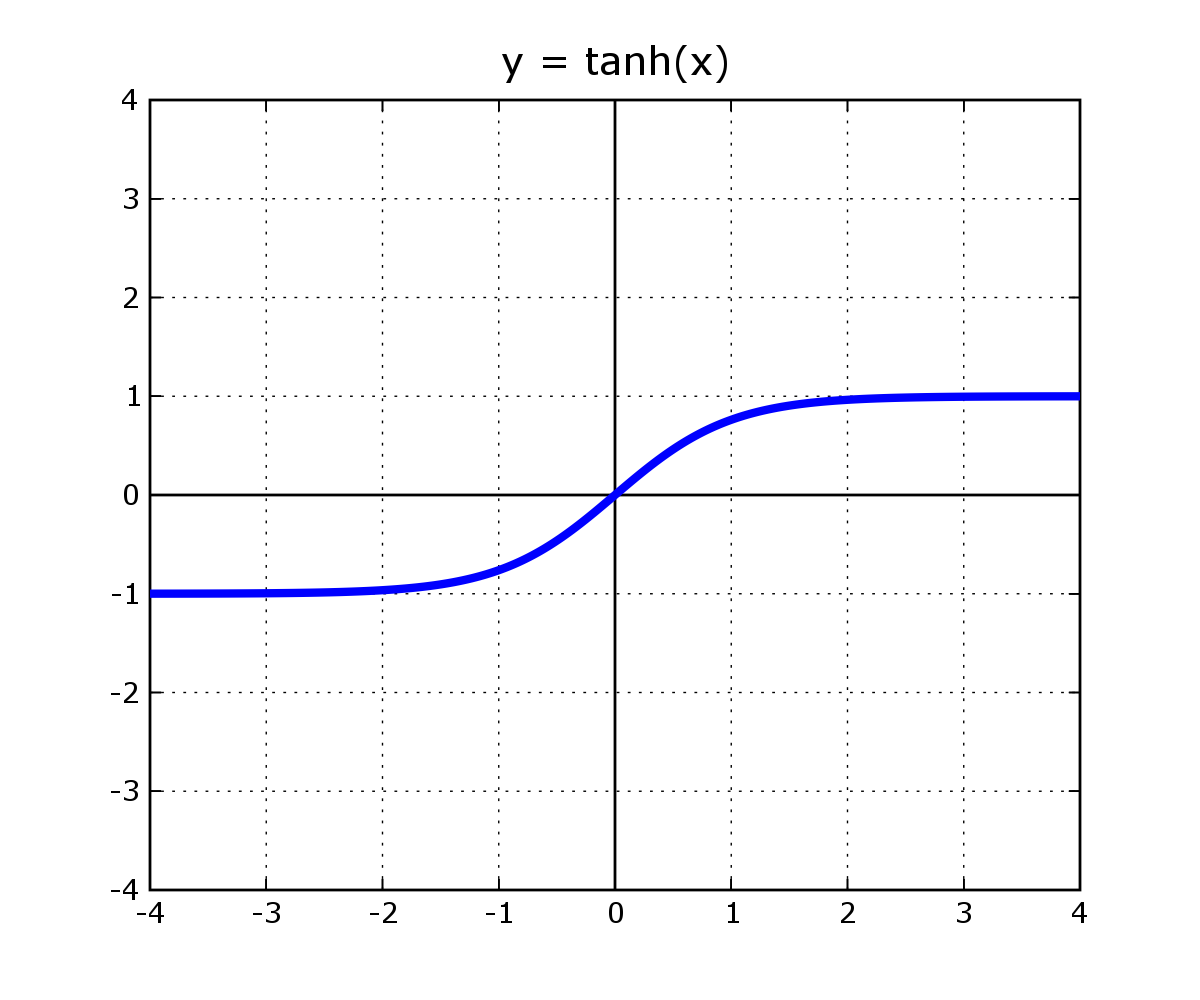
\includegraphics[width=250px]{imgs/tanh_plot.png}
\caption{Hiperbolna tangent funkcija}
\label{fig:tanh_plot}
\end{figure}

Autor u radu \cite{lecun-98b} preporuča korištenje logističke funkcije $f(x) = 1.7159 tanh(\frac{2}{3} x)$. Konstante u navedenoj funkciji su odabrane tako da, ako je ulaz normaliziran, izlazi će isto imati varijancu blizu 1. Konkretni sigmoid ima i sljedeća svojstva: (a) $f(\pm 1) = \pm 1$, (b) druga derivacija ima maksimum u točki $x = 1$.

Logističke funkcije su često definirane izrazima koji sadrže potenciranje prirodnog logaritma $e^{x}, x \in R$, što je računalno prilično zahtjevno. Taj se problem rješava aproksimacijom konkretnog izraza polinomijalnog funkcijom.

% http://web.stanford.edu/~awni/papers/relu_hybrid_icml2013_final.pdf
Drugi je problem nestajući gradijent \engl{vanishing gradient problem}. Nestajući gradijent je pojava koja se događa kada neuroni nekog sloja duboke neuronske mreže imaju gradijente blizu nule jer su izlazi sloja bili blizu zasićenja, odnosno blizu asimptota (koje su često $\pm 1$). Gradijenti blizu nule uzrokuju sporu konvergenciju jer malen iznos gradijenta znači i malu promjenu težina, a pokazalo se i da takve mreže često zaglave u lokalnim minimumima. To su zapravo degenerirani lokalni mimimumi u koje postupak učenja upadne radi korištenja logističkih aktivacijskih funkcija i više se ne može izvući jer je aktivacijska funkcija u zasićenju.

\emph{Rectified linear unit} (kraće ReLU) je vrsta aktivacijske funkcije definirana formulom:
\begin{equation}
f(x) = max(0, x) =
    \left\{
        \begin{array}{ll}
            0  & \mbox{ako } x < 0 \\
            x  & \mbox{ako } x \geq 0
        \end{array}
    \right.
\end{equation}
ReLU rješava oba gore navedena problema: brzo se računa, kao i gradijent (koji je 1, ako je $x > 0$ ili 0) i gradijent nikad ne uđe u zasićenje (uvijek je 1 ili 0), neovisno o dubini mreže.

No, ReLU-ovi imaju i potencijalne mane: ako neki neuron nije aktivan, gradijent je 0, što znači da se težine tog neurona više ne mogu pomaknuti gradijentnom optimizacijom. Tome se problemu može doskočiti postavljanjem početnog pomaka \engl{bias} na neku malu pozitivnu vrijednost (na primjer 0.001), čime će na početku svi neuroni biti aktivirani. Gradijentna optimizacija ih tada može pomicati prema ishodištu (praktički isključiti) ili u pozitivnom smjeru. \cite{maas2013rectifier}

Vjerovalo se i da dobri rezultati, koje ReLU aktivacije postižu u dubokim neuronskim mrežama, potiču i od mogućnosti da ReLU aktivacijska funkcija ''isključi'' neuron (ako vrijednost na ulaza u aktivaciju postane < 0). Rad \cite{xu2015empirical} je pokazao da uspjeh ReLU-a ne leži u gašenju nekih neurona (implicitnom uvođenju rijetke povezanosti). U radu je dana usporedba standardne ReLU funkcije, \emph{leaky ReLU} (lReLU) funkcije, \emph{parametric ReLU} (PRelU) funkcije i \emph{randomized ReLU} (RReLU) funkcije. Eksperimenti su pokazali da funkcije bez nagiba sa smjerom 0 (praktički sve osim standardnog ReLU-a), konzistentno daju bolje rezultate što znači da teorija o gašenju neurone ne vrijedi, jer takve funkcije nikad potpuno ne gase neurone. Pokazano je i da (na manjem skupu podataka) korištenje determinističkog nagiba, ili učenje nagiba na temelju podatka može uzrokovati prenaučenost, naspram funkcije sa slučajnim odabirom nagiba (nagib iz nekog raspona vrijednosti).

\begin{figure}[htb]
\centering
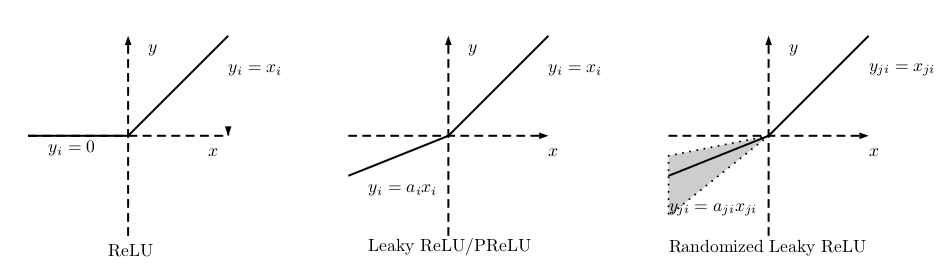
\includegraphics[width=\textwidth]{imgs/relus.png}
\caption{Usporedba ReLU aktivacijskih funkcija}
\label{fig:relu_plot}
\end{figure}

\subsection{Sažimanje}

\textbf{Sažimanje} kod dubokih neuronskih mreža je vrsta poduzorkovanja gdje se ulazna slika (ili mapa značajki) dijeli na više nepreklapajućih pravokutnika i za svaki pravokutnik vrati se jedna vrijednost. Postoji više vrsta sažimanja, a najčešće se koriste sažimanje maksimalnog odziva \engl{max pooling} i sažimanje prosjekom \engl{average pooling}. Primjer sažimanja maksimalnim odzivom prikazan je na slici \ref{fig:max_pooling}.
U slučaju sažimanja maksimalnim odzivom vrijednost koja se vraća za svaki pravokutnik je maksimum svih vrijednosti unutar pravokutnika, dok je kod sažimanja prosjekom to prosječna vrijednost.


Sažimanje maksimalnim odzivom se koristi češće i važno je iz dva razloga:
\begin{enumerate}
    \item smanjuje računsku složenost za gornje slojeve
    \item povećava neosjetljivost na translacije u slici
\end{enumerate}

\begin{figure}[htb]
\centering
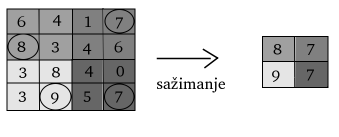
\includegraphics{imgs/max-pooling.png}
\caption{Primjer sažimanja maksimalnim odzivom}
\label{fig:max_pooling}
\end{figure}

Pojasnimo malo povećanje neosjetljivosti na translacije: recimo da se radi sažimanje maksimuma nad regijom od 2x2 piksela. Neka je gornji lijevi piksel onaj s maksimalnom vrijednošću. Ako se sve na slici pomakne za jedan piksel udesno, piksel s maksimalnom vrijednošću će biti gornji desni. To znači da će u oba slučaja izlaz sloja sažimanja maksimuma biti jednak, tj biti će neosjetljiv na takve translacije.

Uobičajena je praksa da se u gornjim slojevima povećava broj mapa značajki. Time bi računalna složenost previše ekspandirala u višim slojevima. Budući da viši slojevi sadrže informacije visoke razine \engl{high level information}, nije važno da su takve informacije dostupne za svaki piksel, dovoljno je da one pokrivaju veće regije slike. Iz tog razloga se poduzorkovanjem u višim slojevima ne gube važne informacije, a uvelike se smanjuje broj operacija i vrijeme potrebno za računanje mapa značajki.

\subsection{Primjer arhitekture}

LeCun je još 1989. godine u radu \cite{lecun-98b}, za klasifikaciju rukom pisanih brojeva na poštanskim pošiljkama, predstavio konvolucijsku mrežu čija arhitektura je začetak današnjih arhitektura. Takva mreža imala je 3 konvolucijska sloja, bez slojeva sažimanja maksimumom, s potpuno povezanim slojem na kraju. Značajan je i LeCun-ov rad \cite{gradient_document} u kojem se predstavlja arhitektura nazvana LeNet, čije inačice se koriste u mnogim verzijama konvolucijskih mrežama.

\begin{figure}[htb]
\centering
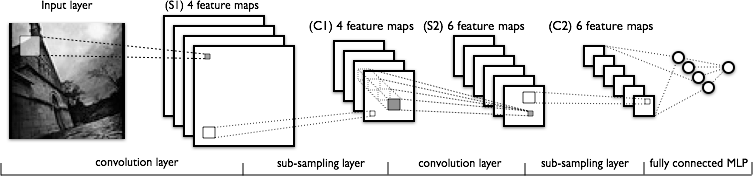
\includegraphics[width=\textwidth]{imgs/mylenet.png}
\caption{LeNet mreža}
\label{fig:lenet5}
\end{figure}
%(slika http://deeplearning.net/tutorial/_images/mylenet.png)

U početnim se slojevima mreže izmjenjuju slojevi sažimanja maksimalnog odziva i mape značajki. Konkretno, prvi sloj se sastoji od 4 mape značajki, zatim slijedi sloj sažimanja maksimuma, pa sloj od 6 mapi značajki i opet sloj sažimanja maksimuma. Zadnji dio takve mreže je višeslojni perceptron na čije su ulaze spojeni izlazi zadnjeg sloja sažimanja maksimuma. Taj se višeslojni perceptron sastoji od 2 sloja. Prvi je skriveni sloj, a iza njega je sloj logističke regresije. Logistička regresija na kraju čini konačnu klasifikaciju. U konkretnom primjeru postoji 10 izlaza, jedan za svaku znamenku.

\chapter{Učenje mreže}

''Učenjem'' modela naziva se postupak pronalaska optimalnih parametara modela. Optimalni parametri su oni koji danim modelom modeliraju skup podataka za učenje, $\mathcal{D}$. $\mathcal{D}$ je skup svih parova $(x_i, y_i)$ gdje je $x_i$ ulazna vrijednost, a $y_i$ izlazna vrijednost. No, modeli se često znaju previše dobro prilagoditi skupu podataka za učenje pa se zapravo relevantni rezultati dobivaju kad se model testira na neviđenim podacima.

Rješenje za optimalne parametre neuronskih mreža nije dostupno u zatvorenoj formi pa se poseže za gradijentnim metodama koje onda kroz iteracije pronalaze optimalne parametre. To znači da nam je potrebna ciljna funkcija, funkcija čiji rezultat nam govori koliko su parametri modela dobri.

Kod klasifikacije slika ulaz u klasifikator je slika, a izlaz je oznaka klase u koju slika pripada. Kod semantičke segmentacije ulaz u klasfikator je opet, ali je izlaz skup oznaka: svaki piksel (ili eventulano grupa piksela) se klasificira pa i svaki ima svoju oznaku. Tako se semantička segmentacija naposljetku zapravo sastoji od višestrukih klasifikacija piksela pa možemo koristiti funkcije gubitka koje koristimo i kod obične klasifikacije.

Najjednostavnija funkcija gubitka je jedan-nula funkcija gubitka. Ako model preslikava ulazni primjer u jedan od razreda iz skupa ${0, ..., L}$, definirajmo takvo preslikvanje funkcijom f $f: R^D \rightarrow {0, ..., L}$, onda se funkcija gubitka može definirati kao:
\begin{equation}
\ell_{0, 1} = \sum_{i = 0}^{\abs{\mathcal{D}}} I_{f(x^{(i)}) \neq y^{(i)}}
\end{equation}
gdje je $\mathcal{D}$ skup podataka, a $I$ indikatorska funkcija definirana kao:
\begin{equation}
I(x) =
    \left\{
	    \begin{array}{ll}
		    1  & \mbox{ako je x istinit} \\
		    0  & \mbox{inače}
	    \end{array}
    \right.
\end{equation}

Budući da jedan-nula gubitak nije derivabilan nije moguće koristiti gradijentnu optimizaciju. Zato se koristi funkcija negativne log izglednosti \engl{negative log likelihood}, spomenuta u poglavlju \ref{chap:logisticka_regresija}.
\begin{equation}
NLL(\theta, \mathcal{D}) = - \sum_{i = 0}^{\abs{\mathcal{D}}} \log P(Y = y^{(i)} | x^{(i)}, \theta)
\end{equation}


\section{Algoritam unazadne propagacije, \emph{engl. backpropagation}}

Algoritmom unazadne propagacije izvode se izrazi za gradijente (iznose derivacija) parametara mreže. Ti se izrazi kasnije koriste u algoritmu gradijentnog spusta za ugađanje parametara.

Algoritam unazadne propagacije prvi je put predstavljen 1970-ih, ali popularnost i prihvaćanje je stekao tek 1986. kad je Hinton izdao poznati rad koji opisuje nekoliko tada poznatih tipova neuronskih mreža i njihovo učenje unazadnom propagacijom koje je bilo brže od prije korištenih metoda učenja i omogućavalo rješavanje problema, koji su do tada bili nerješivi, uz pomoć neuronskih mreža. Do danas je ta metoda učenja postala najproučavanija i nakorištenija.

Slijedi izvod algoritma unazadne propagacije za neuronsku mrežu s $d$ ulaza, $m$ izlaza i $l$ skrivenih slojeva. $l+1$ sloj je izlazni sloj.
Ulaz u sloj $k$ je $\boldsymbol{x}^{(k)}$, a izlaz iz sloja je $\boldsymbol{x}^{(k+1)}$.

Mreža se uči nad skupom za učenje od N parova $(\boldsymbol{x}_i, \boldsymbol{t}_i)$. Vektor $\boldsymbol{x}_i$ je $d$ dimenzionalan, vektor $\boldsymbol{t}_i$ je $m$ dimenzionalan, a $i \in \left\{ 0..N-1 \right\}$. Mreža koristi sigmoidalnu prijenosnu funkciju:
\begin{equation}
  f(\boldsymbol{x}) = \frac{1}{1 + e^{-\boldsymbol{x}}}
\end{equation}
i funkciju gubitka (srednja kvadratna pogreška):
\begin{equation}
  E = \frac{1}{2N} \sum_{n=1}^{N} \sum_{o=1}^{m} \left( t_{n,o} - y_{n,o} \right)^2
    = \frac{1}{2N} \sum_{n=1}^{N} \left( \boldsymbol{t}_{n} - \boldsymbol{y}_{n} \right)^2
\end{equation}
gdje je
\begin{equation} % y(n)
	\boldsymbol{y}_n = \boldsymbol{x}_n^{(l+1)} = f(\boldsymbol{W}^{(l+1)} \boldsymbol{x}_n^{(l)} + \boldsymbol{b}^{(l+1)}) = f(\boldsymbol{net}^{(l+1)})
\end{equation}
\begin{equation} % net(n)
    \boldsymbol{net}^{(k)}_n = \boldsymbol{W}^{(k)} \boldsymbol{x}_n^{(k-1)} + \boldsymbol{b}^{(k)}
\end{equation}

Traže se vrijednosti težina mreže da funkcija $E$ bude minimalna, odnosno želimo izračunati izraz za $\frac{\partial E}{\partial W^{(k)}}$ koji ćemo koristiti kod ugađanja težina:
\begin{equation}
\boldsymbol{W}^{(k)}(t) = \boldsymbol{W}^{(k)}(t-1) - \epsilon \frac{\partial E}{\partial \boldsymbol{W}^{(k)}}(t)
\end{equation}
gdje je $k \in \left\{ 1..l+1 \right\}$, $\boldsymbol{W}^{(k)}$ matrica težina sloja $k$, $t$ je oznaka trenutnog koraka, a $t-1$ oznaka prethodnog koraka.

Parcijalna derivacija funkcije gubitka po težinama za izlazni sloj je:
\begin{equation} % pocetak deriviranja
\begin{split}
  \frac{\partial E}{\partial \boldsymbol{W}^{(l+1)}}
    &= \frac{\partial}{\partial \boldsymbol{W}^{(l+1)}} \left[ \frac{1}{2N} \sum_{n=1}^{N} \left( \boldsymbol{t}_{n} - \boldsymbol{y}_{n} \right)^2 \right] \\
    &= \frac{-1}{N} \sum_{n=1}^{N} \left( \boldsymbol{t}_{n} - \boldsymbol{y}_{n} \right) \frac{\partial \boldsymbol{y}_n}{\partial \boldsymbol{W}^{(l+1)}} \\
    &= \frac{-1}{N} \sum_{n=1}^{N} \left( \boldsymbol{t}_{n} - \boldsymbol{y}_{n} \right) \frac{\partial \boldsymbol{y}_n}{\partial \boldsymbol{net}_n^{(l+1)}} \frac{\partial \boldsymbol{net}_n^{(l+1)}}{\partial \boldsymbol{W}^{(l+1)}}
\end{split}
\end{equation}
U prethodnoj formuli primjenjeno je pravilo ulanjčavanja derivacija: ako je $f$ funkcija od $y$, a $y$ je pak funkcija od $x$, onda vrijedi: $\frac{d f}{d x} = \frac{d f}{d y} \cdot \frac{d y}{d x}$.

Drugi dio formule se raspiše kao:
\begin{equation}  % net / W
\label{eq:parc_net_over_parc_w}
  \frac{\partial \boldsymbol{net}_n^{(l+1)}}{\partial \boldsymbol{W}^{(l+1)}}
    = \frac{\partial}{\partial \boldsymbol{W}^{(l+1)}} \left[ \boldsymbol{W}^{(l+1)} \boldsymbol{x}_n^{(l)} + \boldsymbol{b}^{(l+1)} \right]
    = \boldsymbol{x}_n^{(l)}
\end{equation}

Budući da je $\boldsymbol{y}_n = f(\boldsymbol{net}_n^{(l+1)} )$, gdje je $f$ logistička funkcija čija je derivacija $f'(x) = f(x) [1 - f(x) ]$, slijedi da je:
\begin{equation} % d y / d net
  \frac{\partial \boldsymbol{y}_n}{\partial \boldsymbol{net}_n^{(l+1)}}
    = f'\left(\boldsymbol{net}_n^{(l+1)}\right)
    = f\left(\boldsymbol{net}_n^{(l+1)}\right) \left[ 1 - f\left(\boldsymbol{net}_n^{(l+1)}\right) \right]
\end{equation}
iz čega se dobije:
\begin{equation}
\begin{split}
  \frac{\partial E}{\partial \boldsymbol{W}^{(l+1)}}
    &= \frac{-1}{N} \sum_{n=1}^{N} \left( \boldsymbol{t}_{n} - \boldsymbol{y}_{n} \right) f'\left(\boldsymbol{net}_n^{(l+1)}\right) \boldsymbol{x}_n^{(l)} \\
    &= \frac{-1}{N} \sum_{n=1}^{N} \delta_n^{(l+1)} \boldsymbol{x}_n^{(l)}
\end{split}
\end{equation} % delta (l+1)
gdje se $\delta_n^{(l+1)}$ definira kao:
\begin{equation} 
\label{eq:delta_lastlayer}
  \delta_n^{(l+1)}
    = \left( \boldsymbol{t}_{n} - \boldsymbol{y}_{n} \right) f'\left(\boldsymbol{net}_n^{(l+1)}\right)
\end{equation}
a $\boldsymbol{x}_n^{l}$ je ulaz u izlazni sloj.

Uzmimo sada za primjer matricu težina nekog skrivenog sloja $l$. Izvod započinje slično:
\begin{equation} % zapocinje izvod za skriveni sloj dE / dW
\label{eq:e_over_w_hidden_layer}
\begin{split}
  \frac{\partial E}{\partial \boldsymbol{W}^{(l)}}
    &= \frac{\partial}{\partial \boldsymbol{W}^{(l)}} \left[ \frac{1}{2N} \sum_{n=1}^{N} \left( \boldsymbol{t}_{n} - \boldsymbol{y}_{n} \right)^2 \right] \\
    &= \frac{-1}{N} \sum_{n=1}^{N} \left( \boldsymbol{t}_{n} - \boldsymbol{y}_{n} \right) \frac{\partial \boldsymbol{y}_n}{\partial \boldsymbol{W}^{(l)}} \\
    &= \frac{-1}{N} \sum_{n=1}^{N} \left( \boldsymbol{t}_{n} - \boldsymbol{y}_{n} \right) \frac{\partial \boldsymbol{y}_n}{\partial \boldsymbol{net}_n^{(l+1)}} \frac{\partial \boldsymbol{net}_n^{(l+1)}}{\partial \boldsymbol{W}^{(l)}}
\end{split}
\end{equation}

Izraz $\frac{\partial \boldsymbol{net}_n^{(l+1)}}{\partial \boldsymbol{W}^{(l+1)}}$ smo već derivirali u \ref{eq:parc_net_over_parc_w}, a izraz $\frac{\partial \boldsymbol{net}_n^{(l+1)}}{\partial W^{(l)}}$ deriviramo kao:
\begin{equation} % d net / d W
\begin{split}
  \frac{\partial \boldsymbol{net}_n^{(l+1)}}{\partial W^{(l)}}
    &= \frac{\partial}{\partial \boldsymbol{W}^{(l)}} \left[ \boldsymbol{W}^{(l+1)} \boldsymbol{x}_n^{(l)} + \boldsymbol{b}^{(l+1)} \right] \\
    &= \boldsymbol{W}^{(l+1)} \frac{\partial \boldsymbol{x}_n^{(l)}}{\partial W^{(l)}} \\
    &= \boldsymbol{W}^{(l+1)} \frac{\partial f \left( \boldsymbol{net}_n^{(l)} \right) }{\partial W^{(l)}} \\
    &= \boldsymbol{W}^{(l+1)} \frac{\partial f \left( \boldsymbol{net}_n^{(l)} \right)}{\partial \boldsymbol{net}_n^{(l)}} \frac{\partial \boldsymbol{net}_n^{(l)}}{\partial W^{(l)}} \\
    &= \boldsymbol{W}^{(l+1)} f'\left(\boldsymbol{net}_n^{(l)}\right) \boldsymbol{x}_n^{(l-1)}
\end{split}
\end{equation}

Kad to uvrstimo natrag u izraz \ref{eq:e_over_w_hidden_layer} dobijemo:
\begin{equation}
  \frac{\partial E}{\partial \boldsymbol{W}^{(l)}}
    = \frac{-1}{N} \sum_{n=1}^{N} \left( \boldsymbol{t}_{n} - \boldsymbol{y}_{n} \right) f'\left(\boldsymbol{net}_n^{(l+1)}\right) \boldsymbol{W}^{(l+1)} f'\left(\boldsymbol{net}_n^{(l)}\right) \boldsymbol{x}_n^{(l-1)}
\end{equation}
što se može kraće zapisati kao:
\begin{equation}
  \frac{\partial E}{\partial \boldsymbol{W}^{(l)}}
    = \frac{-1}{N} \sum_{n=1}^{N} \delta_n^{(l)} \boldsymbol{x}_n^{(l-1)}
\end{equation}
gdje je $\delta^{(l)}$ jednak:
\begin{equation} % delta (l)
\label{eq:delta_hiddenlayer}
  \delta^{(l)}
    = \delta^{(l+1)} \boldsymbol{W}^{(l+1)} f'\left(\boldsymbol{net}_n^{(l)}\right)
\end{equation}
a $l$ je proizvoljni skriveni sloj.

Ako je aktivacijska funkcija $f$ logistički sigmoid onda se to može dalje raspisati kao:
\begin{equation}
  \delta^{(l)}
    = \delta^{(l+1)} \boldsymbol{W}^{(l+1)} f\left(\boldsymbol{net}_n^{(l)}\right) \left[ 1 - f\left(\boldsymbol{net}_n^{(l)}\right) \right]
\end{equation}

Vidi se da su izrazi za $\frac{\partial E}{\partial W^{(l)}}$ jednaki:
\begin{equation}
  \frac{\partial E}{\partial \boldsymbol{W}^{(k)}}
    = \frac{-1}{N} \sum_{n=1}^{N} \delta_n^{(k)} \boldsymbol{x}_n^{(k-1)}
\end{equation}
gdje je $k$ ili skriveni ili izlazni sloj. Drugačiji je samo način na koji se računa $\delta^{(k)}$. Za zadnji sloj se koristi izraz \ref{eq:delta_lastlayer}, dok se za skriveni sloj koristi izraz \ref{eq:delta_hiddenlayer} koji koristi već izračunati $\delta_n$ idućeg sloja. Upravo se zato algoritam naziva ''algoritam unazadne propagacije'' jer se kreće od zadnjeg (izlaznog sloja) i pogreška, odnosno podešavanje težina, se propagira prema prvom (ulaznom) sloju.

\section{Gradijentni spust}

Gradijentni spust je optimizacijski algoritam, odnosno algoritam pronalaska minimuma derivabilne konveksne funkcije. Algoritam gradijentnog spusta traži lokalni minimum na način da u trenutnoj točki traži smjer gradijenta funkcije i zatim napravi pomak u negativnom smjeru gradijenta. Ako je korak dovoljno malen, nova vrijednost trenutne točke će biti manja od prethodna.
U slučaju da je pomak prevelik, nema garancije da ćemo se pomaknuti u točku u kojoj je vrijednost funkcije manja, već postoji mogućnost da se pomaknemo na suprotnu padinu funkcije i zapravo povećamo vrijednost funkcije u trenutnoj točki.

Neka je $f(x)$ funkcija čiji minimum tražimo, $A$ trenutna točka, $t$ je trenutni korak, a $t-1$ je prethodni korak. Jedna iteracija algoritma je onda:
\begin{equation}
  A(t) = A(t-1) - \eta f' \left[ A(t-1) \right]
\end{equation}
ili za funkciju $F$ s više parametara:
\begin{equation}
  \boldsymbol{A}_i(t) = \boldsymbol{A}_i(t-1) - \eta \frac{\partial F}{\partial \boldsymbol{A}_i} \left[ \boldsymbol{A}_i(t-1) \right]
\end{equation}
gdje je indeks $i$ označava $i$-tu komponentu vektora, konstanta $\eta$  označava korak algoritma, odnosno to je konstanta koja će pomnožena s iznosima gradijenata dati iznos pomaka.

Pod uvjetom da je $\eta$ dovoljno malen, biti će $f(a(t)) < f(a(t-1))$, odnosno pomaknut ćemo se u točku koja je bliže minimumum funkcije.

Kod neuronskih mreža funkcija koju optimiramo je funkcija gubitka $E$, a točka koju pomičemo je višedimenzionalna točka čija svaka dimenzija predstavlja jednu težinu neuronske mreže.

Da bi se algoritam gradijentnog spusta mogao koristiti za podešavanje težina u neuronskim mrežama, potrebno je derivirati funkciju gubitka. Kao prvo, nužno je da je ona derivabilna što je slučaj kod negativne log-izglednosti:
\begin{equation}
  \frac{\partial \mathcal{L}(x | \theta)}{\partial \theta_{ij}}
  	= \partial \left[ - \sum_{x \in D} ln P (y|x) \right] / \partial \theta_{ij}
    = - \sum_{x \in D} \frac{1}{P(y|x)} \frac{\partial P(y|x)}{\partial \theta_{ij}}
\end{equation}
Budući da je $P(y|x)$ izlaz neuronske mreže, koji je derivabilan ako je prijenosna funkcija derivabilna, vidi se da je cijeli izraz derivabilan.

\subsection{Stohastički gradijentni spust}

Obično se koristi metoda gradijentnog spusta nazvana stohastički gradijentni spust. Neka je $E_n(w)$ vrijednost funkcije gubitka na n-tom primjeru za neke parametre $w$.

Kada bi za minimizaciju koristili standardni (ili ''grupni'') gradijentni spust, jedna bi iteracija izgledala ovako:
\begin{equation}
    \boldsymbol{w}(t) = \boldsymbol{w}(t-1) - \eta \nabla E(\boldsymbol{w}(t)) = \boldsymbol{w} - \eta \sum_{n=1}^N \nabla E_i(\boldsymbol{w}),
\end{equation}
gdje je $\eta$ korak učenja (često zvan i stopa učenja).

U mnogo slučajeva, funkcija nad kojom se vrši zbrajanje ima jednostavan oblik koji omogućava brzo izračunavanje zbrajanje i cijelog izraza.

No, postoje funkcije kod kojih izračuvanje sume u gradijentu zahtijeva dugotrajne izračune. Kad je skup za treniranje velik, to postaje problem. Da bi se ubrzalo izvođenje izračuna, u svakoj iteraciji se izvodi gradijenti spust, odnosno izračun funkcije gradijenta. Takvim se postupkom aproksimira pravi gradijent funkcije gubitka gradijentom jednog primjera (jedne iteracije):
\begin{equation}
    \boldsymbol{w}(t) = \boldsymbol{w}(t-1) - \eta \nabla E_n(\boldsymbol{w}(t)).
\end{equation}
Prolazom algoritma kroz skup za treniranje izvodi se gornje podešavanje težina za svaki primjer. Potrebno je nekoliko prolaza kroz skup za treniranje dok algoritam ne konvergira. Tipične implementacije još i promješaju skup za učenje prije svakog prolaza.

Ako je skup podataka velik i jako redundantan, gradijent na prvoj polovici skupa je skoro identičan gradijentu na drugoj polovici skupa. Umjesto računanja gradijenata za cijeli skup podataka, težine mreže se mogu ugoditi nakon računanja gradijenata za svaku polovicu skupa. Ako dijeljnjem skupa podataka odemo u krajnost, dolazimo do stohastičkog gradijentnog spusta (nazivan još i \emph{online} učenje) gdje se težine ugađaju nakon svakog primjera iz skupa za učenje, čime se konvergencija ubrzava jer nije potrebno računati gradijent svih uzoraka da bi došlo do ugađanja težina.

Za većinu problema najboljim se pokazalo učenje korištenjem male serije skupa podataka \engl{mini-batch learning}. Budući da je ugađanje težina mreže računalno skupo, takva metoda učenje je brža od običnog stohastičkog gradijentnog spusta jer nema ugađanja težina nakon svakog primjera. Do ubrzavanja dolazi i jer se kod računanja gradijenata za seriju primjera koristi puno matričnog množenja koje je u današnjim arhitekturama računalnih sustava jako efikasno, pogotovo ako se koriste grafičke kartice.

Važno je i napomenuti da računanje gradijenata na dijelu podataka (\textit{mini-batch} i stohastički gradijentni spust) svodi na aproksimaciju gradijenta cijelog skupa podataka, odnosno unosimo šum u račun gradijenata.
Taj šum je koristan u optimizaciji jer pomaže da se postupak izvuče iz eventualnog lokalnog mimimuma u kojem zapeo. \textit{Mini-batch} učenje je zato dobar kompromis između memorijskih zahtjeva i brzine konvergencije.


\subsection{\emph{Momentum} metoda}

Za višeslojne neuronske mreže višedimenzionalna ravnina funkcije pogreške je kompliciranog oblika, ali se lokalno može aproksimirati kao kvadratna posuda. Njen vertikalni presjek je onda parabola, a horizontalni elipsa.

(slika)

Uzmimo za primjer kretanje loptice na takvoj funkciji pogreške. Loptica će krenuti u smjeru lokalnog gradijenta, ali jednom kad nakupti brzinu ići će više u smjeru centra kvadratne posude nego u smjeru gradijenta. Njen moment će je natjerati da ide u smjeru ovisnom o prethodnom kretanju.

Slična je stvar i s \emph{momentum} metodom koja uzima u obzir gradijente prethodnih koraka i tako prigušuje oscilacije u promjeni smjera, a povećava brzinu u smjeru konzistentnih gradijenata.

Gradijenti imaju utjecaj na povećanje prethodne brzine (konstanta $\alpha$ polako smanjuje brzinu, ima iznos malo manji od 1, često 0.9):
\begin{equation}
\boldsymbol{v}(t) = \alpha \boldsymbol{v}(t-1) - \eta \frac{\partial E}{\partial \boldsymbol{w}}(t)
\end{equation}

Promjena težina je ekvivalentna trenutnoj brzini:
\begin{equation}
\begin{split}
	\Delta \boldsymbol{w}(t) &= \boldsymbol{v}(t) \\
		&= \alpha \boldsymbol{v}(t-1) - \eta \frac{\partial E}{\partial \boldsymbol{w}}(t) \\
		&= \alpha \boldsymbol{w}(t-1) - \eta \frac{\partial E}{\partial \boldsymbol{w}}(t)
\end{split}
\end{equation}

\subsection{Resilient propagation (RProp)}

Rprop metoda, poput stohastičkog gradijentnog spusta, koristi lokalne gradijente da bi ugodila parametre težina mreže. Razlika je da se za Rprop koristi samo predznak  derivacija, što znači da je veličina koraka neovisna o amplitudi gradijenta. Ova metoda se koristi samo kod ugađanja težina nakon svih viđenih primjera iz skupa za učenje \engl{full batch learning}.

Postoji više varijanti RProp algoritma: RProp+, RProp-, iRPop+, iRPRop- (\cite{Igel00}).
Znak + ili - na kraju naziva označava prati li algoritam prethodnu promjenu težina $\Delta w_{ij}$ \engl{weight backtracking} -- ako prati, onda se promjenom smjera gradijenata poništava prethodna promjena težina. $i$ na početku naziva označava postupak gdje se kod promjene smjera gradijenata trenutna vrijednost postavlja na 0: $ako \ \frac{\partial E}{\partial w_{ij}}(t) * \frac{\partial E}{\partial w_{ij}}(t-1) < 0 \rightarrow \frac{\partial E}{\partial w_{ij}}(t) := 0$

U nastavku će biti opisana iRProp- varijanta \cite{Igel00} koja se često koristi. Budući da promjena težina ne ovisi o iznosu gradijenta, definiraju se ''vrijednosti promjene'' za čiji iznos se podešavaju težine:
\begin{equation}
  \Delta w_{ij}(t) =
    \left\{
	    \begin{array}{ll}
		    -\Delta_{ij}(t)  & \mbox{ako} \frac{\partial E}{\partial w_{ij}}(t) > 0 \\
		    +\Delta_{ij}(t)  & \mbox{ako} \frac{\partial E}{\partial w_{ij}}(t) < 0\\
		    0  & \mbox{inače}
	    \end{array}
    \right.
\end{equation}
gdje $\frac{\partial E}{\partial w_{ij}}(t)$ označava sumu gradijenata za sve primjere.

Drugi korak postupka je određivanje novih ''vrijednosti promjene'' $\Delta_{ij}(t)$ za svaki parametar mreže (svaku težinu i pristranost).
\begin{equation}
  \Delta{ij}(t) =
    \left\{
	    \begin{array}{ll}
		    \eta^{+} * \Delta_{ij}(t-1)  & \mbox{ako} \frac{\partial E}{\partial w_{ij}}(t) * \frac{\partial E}{\partial w_{ij}}(t-1) > 0 \\
		    \eta^{-} * \Delta_{ij}(t-1)  & \mbox{ako} \frac{\partial E}{\partial w_{ij}}(t) * \frac{\partial E}{\partial w_{ij}}(t-1) < 0\\
		    \Delta_{ij}(t-1)  & \mbox{inače}
	    \end{array}
    \right.
\end{equation}
gdje je $0 < \eta^{-} < 1 < \eta^{+}$. Često se u implementacijama koriste vrijednosti $\eta^{-} = 0.5$ i $\eta^{+} = 1.2$.

Ili rječima: svaki put kada parcijalna derivacija neke težine promjeni predznak, što znači da je prošlo ugađanje težina bilo preveliko i preskočio se lokalni minimum, ''vrijednost promjene'' se smanji s faktorom $\eta^{-}$. Ako se predznak nije promijenio, ''vrijednost promjene'' se lagano uveća s faktorom $\eta^{+}$, tako da postupak akcelerira po plitkim područjima.

Pojasnimo na primjeru zašto Rprop ne radi dobro kod stohastičkog gradijentog spusta (ugađanja težina nakon svakog primjera). Neka jedna težina mreže ima gradijent +0.1 na devet primjera i gradijent od -0.9 na jednom primjeru. Tada želimo da ta težina ostane otprilike ista, a Rprop će povećati težinu devet puta i smanjiti jednom za otprilike isti iznos.


\subsection{RMS prop}

\emph{Rmsprop} metoda, kao i stohastički gradijentni spust koristi malene lokalne pomake da bi ugodila težine, a prvenstveno se koristi kod \textit{mini-batch} učenja.
Podskup podataka u trenutnoj iteraciji može imati primjere za učenje skroz drugih klasa od prethodne iteracije što će uvelike promijeniti iznose gradijenata. Da bi se ublažile takve promjene koristi se pomični prosjek gradijenata koji ih zagladi.
\emph{Rmsprop} to zaglađivanje provodi tako da kod računanja gradijenata u svakom koraku računa i eksponencijalni pomični prosjek \engl{exponential moving average, EMA} kvadrata gradijenata. Za svako ugađanje, EMA se koristi kako bi se izračunao korijen iz srednjih kvadrata \engl{root mean square, RMS} vrijednosti gradijenata koji su dobiveni u prošlim koracima. Trenutna vrijednost gradijenata se zatim podijeli s korijenom srednjih kvadrata.

Neka je gradijent neke težine $\boldsymbol{W}$ definiran s $\boldsymbol{grad} = \frac{\partial E}{\partial \boldsymbol{W}}$. Eksponencijalni pomični prosjek gradijenata onda možemo definirati s:
\begin{equation}
  \boldsymbol{s}(t) = \aleph \cdot \boldsymbol{s}(t-1) + (1 - \aleph) \cdot \boldsymbol{grad}^2
\end{equation}
Opisana varijanta Rmspropa \cite{Graves13} koristi i \emph{momentum} metodu ugrađenu u sam postupak Rmspropa.
\begin{equation} % v
  \boldsymbol{v}(t) = \alpha \boldsymbol{v}(t-1) - \eta \frac{\boldsymbol{grad}}{\sqrt{\boldsymbol{s} + \epsilon}}
\end{equation}
\begin{equation} % w
  \Delta \boldsymbol{W}(t) = \boldsymbol{v}(t)
\end{equation}
gdje je $s$ trenutni iznos eksponencijalnog pomičnog prosjeka, $\aleph$ je konstanta eksponencijalnog pomičnog prosjeka (koristi se vrijednost 0.95),  $\boldsymbol{v}$ je trenutna brzina, $\alpha$ je \emph{momentum} konstanta, $\eta$ je stopa učenja (koristi se vrijednost 0.001), $W$ je matrica težina nekog sloja, a $\epsilon$ je konstanta koja sprječava dijeljenje s nulom.


\section{Regularizacija}

Regularizacija je često korištena tehnika u strojnom učenju, a odnosi se na postupak pružanja dodatnih informacija funkciji gubitka kako bi se rješio problem šuma u ulaznom skupu podataka i problem prenaučenosti. Prenaučenost je pojava tijekom učenja modela kad se model prilagodi skupu za učenje u tolikoj mjeri da točnost na skupu za provjeru \engl{validation set} počne padati, iako se točnost na skupu za učenje povećava.

Regularizacijom se sprječava da se model previše prilagodi skupu za učenje tako da pogreška na neviđenim podacima bude manja (skupu za provjeru) iako se pogreška na skupu za učenju još može smanjiti. U idućim poglavljima navedene su najčešće tehnike za regularizaciju modela dubokih neuronskih mreža.

\subsection{$L_1$ i $L_2$ regularizacija}

$L_1$ norma je suma apsolutnih iznosa kartezijevih komponenti vektora. Drugačije gladajući, $L_1$ norma se definira kao suma projekcija vektora na koordinatne osi. Za neki vektor $\boldsymbol{x}$ se $L_1$ norma definira kao:
\begin{equation}
\norm{\boldsymbol{x}}_1 = \sum_{i = 1}^{n} \abs{x_i}
\end{equation}

$L_2$ norma je suma kvadrata komponenti vektora. Za neki vektor $\boldsymbol{x}$ se ona definira:
\begin{equation}
\norm{\boldsymbol{x}}_2 = \sum_{i = 1}^{n} {x_i}^2
\end{equation}

Tijekom učenja modela, želimo modelom što bolje modelirati podatke nad kojima učimo, no pravi je cilj da model radi dobro na neviđenim primjerima (primjeri koje nije vidio tijekom učenja). Pojasnimo na primjeru logističke regresije što se događa ako učenje predugo traje: budući da funkcija negativne log izglednosti asimptotski teži prema nuli, optimizacija nikada neće završiti, a dogodit će se da neke težine u mreži stalno rastu jer tim rastom uzrokuju polagano padanje negativne izglednosti na skupu za učenje. Jednaka stvar se događa i u neuronskim mrežama, gdje je broj težina još puno veći.

Tom rastu se može doskočiti tako da se norma vektora uključi u funkciju gubitka. Funkcija $R$ označava normu vektora težina mreže. Regularizirana funkcija gubitka je onda:
\begin{equation}
    E(\theta, \mathcal{D}) = NLL(\theta, \mathcal{D}) + \lambda R(\theta) = \\
    = NLL(\theta, \mathcal{D}) + \lambda \norm{\theta}_p^p
\end{equation}
gdje je
\begin{equation}
    \norm{\theta}_p = (\sum_{j = 0}^{\abs{\theta}} \abs{\theta_j}^p)^{\frac{1}{p}}
\end{equation}
$p$ je najčešće 1 ili 2, odnosno koristi se $L_1$ ili $L_2$ norma. $\lambda$ je regularizacijski faktor, jedan od hiperparametara mreže, koji se određuje eksperimentalno.

\subsection{Slučajne transformacije ili Umjetno povećanje skupa za učenje}
\label{chap:dataset_perturbations}

Kod modela s velikim brojem parametara, kao što su duboke neuronske mreže, veličina skupa za učenje uvelike utječe na rezultate: što je veći skup za učenje, to su bolji rezultati na skupu za testiranje jer je bolja generalizacija modela. No, veličina skupa za učenje je uvijek ograničena. Kod semantičke segmentacije broj podataka je još više ograničen jer je sam postupak označavanja slika semantičkim oznakama dugotrajan pa time i skup.
Zato se provodi postupak umjetnog ''povećanja'' skupa za učenja slučajnim transformacijama.

Kod računalnog vida, koji se većinom bavi slikama, slučajne transformacije su obično:
\begin{itemize}
  \item
  	\textbf{translacije} slike po x ili y osi za neki malen pomak, na primjer 5\% slike
  \item
    \textbf{rotacije} slike za kut od $\pm 7\deg$
  \item
  	\textbf{skaliranje} (uvećavanje ili smanjivanje) slike za neki faktor koji je obično u raponu od <0.9, 1.1>
  \item
    \textbf{smik} slike za kut od$\pm 5\deg$
\end{itemize}

Slučajne transformacije se koriste tako da se za svaku sliku prvo odabere podskup transformacija koje će se koristiti na toj slici, a zatim se slučajno odabiru parametri svake od odabranih transformacija.

Jedan način korištenja je da se pomoću navednih funkcija unaprijed generira povećana verzija skupa podataka, a drugi da se transformacije provode ''uživo'', odnosno prije svake epohe treniranja. Tijekom provođeja transformacija ''uživo'' mreža se nikad ne trenira s istom slikom dva puta. Svaki put mreža ''vidi'' drugu verziju (transformiranu) iste slike čime se uvelike sprječava pretreniranost i prevelika prilagodba na skup za učenje.

\subsection{Dropout}

Točnost predikcije raznih modela čije treniranje počinje sa slučajno inicijaliziranim parametrima, se povećava ako se koristi prosjek predikcija više istrenranih modela. Takav način korištenja gotovih modela se naziva uprosječivanje modela \engl{model averaging}. No, mane takvog pristupa su (i )što treniranje svake mreže traje dugo i (ii) ne želimo tijekom korištenja pokretati više modela za isti primjer jer to opet dugo traje što je pogotovo loše za primjenu u realnom vremenu.

\emph{Dropout} je metoda za učinkovito uprosječivanje modela velikih neuronskih mreža\cite{hinton_dropout}. Uzmimo za primjer jedan skriveni sloj na kojem čemo primjeniti \emph{dropout} metodu. Svaki puta kad mreži na ulaz postavimo jedan primjer iz skupa za učenje, slučajno ''ugasimo'' svaki neuron s vjerojtnošću $p$ (za skrivene slojeve najčešće je $p = 0.5$, odnosno ''ugasimo'' polovicu neurona. ''Gašenjem'' se smatra postavljanje izlaza određenog neurona na 0. To zapravo znači da slučajno odabiremo jednu od $2^H$ arhitektura mreže, gdje je $H$ broj neurona u skrivenom sloju, a sve arhitekture dijele iste težine. Dijeljenje težina između velikog broja arhitektura, odnosno modela, je zapravo jaka regularizacija mreže. Budući da postoji velik broj arhitektura, svaka će pojedina arhitektura vidjeti samo nekolicinu primjera.

Ostaje još za odgovoriti što se događa tijekom testiranja modela (ili korištenja). Prva ideja je odabrati nekoliko različitih arhitektura, napraviti njihove predkcije i uprosječiti ih. No, brži način je koristiti sve neurone skrivenog sloja, a njihove izlaze onda pomnožiti s $p$. Može se pokazati da je to jednako računanju geometrijske sredine predikcije svih $2^H$ modela.

Kod mreža s više slojeva, \emph{dropout} kod ulaznih slojeva je manji, koristi se $p = 0.9$ (samo 10\% ulaznih neurona se gasi). Neki autori navode da koriste u svim skrivenim slojevima $p = 0.5$, dok neki postepeno smanjuju $p$ od 0.9 (na ulazu), do 0.5 u zadnjem skrivenom sloju.

Ako se duboka mreža lako prenauči, \emph{dropout} će osjetno smanjiti grešku. No, ako se mreža ne može prenaučiti, onda je potrebno koristiti mrežu s više parametara (širu ili dublju).
% Hinton: nips2012_hinton_networks_01.pdf


\chapter{Semantička segmentacija}

Semantička segmentacija je proces pridavanja labele svakom pikselu slike. Labele su obično oznake objekata koji su predstavljeni slikom.
Semantička segmentacija spaja klasične probleme detekcije objekata, segmentacije slika i višeklasne klasifikacije u jedan proces.

Prepoznavanje nekog tipa objekta na slici se uglavnom temelji na tome da tražimo objekte slične teksture i sličnih obrisa, ali ponekad niti te dvije stvari ne govore točno koji je to objekt. Takvi zadaci znaju biti teški i za ljudske označivače, stoga automatizacija takvog zadatka računalima nije nimalo jednostavna.

Postavljaju se dva vrlo važna pitanja: kako dobro prikazati slikovne informacije u sustavu za označavanje scene i kako te informacije iskoristiti za interpretaciju. Budući da je ideja konvolucijskih mreža da rade kao detektori značajki, konvolucijske mreže se u praksi koriste i za izvlačenje značajki i za klasifikaciju.

Razumijevanje scena je jako važno kod mnogih primjena, a posebno kod robotike. Jedan od važnih ciljeva u području robotike je omogućiti robotima da se autonomno kreću kroz prostor koji dijele s ljudima. Najvažnija stvar u implementaciji takvog sustava je prepoznavanje i intepretacija okoline.


\section{Testni skupovi}

Ulaz u sustav koji provodi semantičku segmentaciju obično je RGB ili RGBD slika (D označava komponentu dubine). Prije samog modela takve se slike znaju pretprocesirati, recimo iz RGB u YUV komponenete, a ponekad u model ulaze i bez ikakvog procesiranja. Podaci koje sustav koristi za učenje su semantičke oznake: one mogu biti u obliku slika određenog podskupa boja, gdje svaka boja predstavlja neku oznaku ili u tekstualnom formatu gdje je za svaki piksel spremljen indeks njegove oznake. U nastavku su opisani korišteni skupovi podataka.


\subsection{Stanford Background Dataset}

\textit{Stanford Background Dataset}\cite{gould_09} je skup podataka za geometrijsko i semantičko razumijvanje scene. U sklopu ovog rada korištene su isključivo semantičke oznake scene. Skup podataka se sastoji od 715 slika skupljenih iz raznih skupova podataka: \textit{MSRC}, \textit{LabelME}, \textit{PASCAL VOC} i \textit{Geometric Context}. Sve slike su veličine oko 320 x 240 piksela, uz odstupanja od desetak piksela, i prikazuju vanjske scene.
U skupu postoji 8 semantičkih oznaka: nebo, stablo, cesta, trava, voda, zgrada, planina, glavni objekt i oznaka ''nepoznato''. Semantičke oznake su spremljene u tekstualnim datotekama gdje broj u retku $y$ i stupcu $x$ (stupci su odojeni razmacima) predstavlja indeks oznake piksela na lokaciji $(x, y)$

\begin{bchart}[step=5,max=40,unit=\%]
    \bcbar[label = nepoznato]{2.8}
      \smallskip
    \bcbar[label = nebo]{22.8}
      \smallskip
    \bcbar[label = stablo]{7.4}
      \smallskip
    \bcbar[label = cesta]{18.2}
      \smallskip
    \bcbar[label = trava]{4.9}
      \smallskip
    \bcbar[label = voda]{12.1}
      \smallskip
    \bcbar[label = zgrada]{15.0}
      \smallskip
    \bcbar[label = planina]{2.0}
      \smallskip
    \bcbar[label = prednji objekt]{14.8}
	\bcxlabel{zastupljenost oznake}
\end{bchart}

\begin{figure}[htb]
\centering
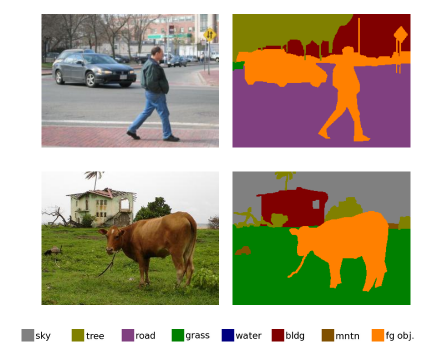
\includegraphics[width=350px]{imgs/dag-example.png}
\caption{Primjer slike i oznaka Stanford Background skupa podataka}
\label{fig:stanford_dataset}
\end{figure}

\subsection{KITTI}
KITTI\footnote{\emph{http://www.cvlibs.net/datasets/kitti/}} je projekt pokrenut od strane dva instituta: Karslruhe Institue of Technology i Toyota Technological Institute, odakle dolazi i naziv. U sklopu toga projekta napravljen je veliki skup podataka koji se sastoji od slika s kamere, stereo kamera, GPS zapisa i laserskih snimki, prikupljenih s automobila u vožnji. Od tih podataka je napravljeno nekoliko skupova
podataka za određene probleme poput rekonstrukcija putanje pomoću kamera, stereoskopske rekonstrukcije, detekcije objekta, prepoznavanja objekata i slično.

Ros et al.\cite{ros:2015} su odabrali određene slike s kamere i semantički ih označili. Taj se skup slika sastoji od 146 označenih slika, od čega je 100 slika skup za učenje i njih 46 skup za testiranje. Slike su veličine 1241 x 376 piksela.
Semantičke oznake skupa su: nebo, zgrada, cesta, pločnik, ograda, vegetacija, stup, auto, znak, pješak i biciklist. Oznake su spremljene kao posebne slike (jednakih veličina kao i ulazne) gdje određena boja u slici predstavlja pojedinu oznaku.
Učenje otežava činjenica da su neke oznake jako slabo zastupljene jer mreža puno sporije uči primjere čijih je oznaka malo i slabo ih može generalizirati.
Konvolucijska mreža je na ovom skupu podataka isprobana u dvije inačice: prva inačica je primala na ulaz samo RGB podatke, dok je druga inačica osim RGB slike primala i dubinsku mapu prostora dobivenu stereoskopskom rekonstrukcijom.

\begin{bchart}[step=5,max=40,unit=\%]
    \bcbar[label = nepoznato]{1.4}
      \smallskip
    \bcbar[label = zgrada]{32.1}
      \smallskip
    \bcbar[label = vegetacija]{22.4}
      \smallskip
    \bcbar[label = cesta]{15.5}
      \smallskip
    \bcbar[label = automobil]{13.3}
      \smallskip
    \bcbar[label = pločnik]{5.8}
      \smallskip
    \bcbar[label = nebo]{4.5}
      \smallskip
    \bcbar[label = ograda]{3.1}
      \smallskip
    \bcbar[label = stup]{0.4}
      \smallskip
    \bcbar[label = biciklist]{0.2}
      \smallskip
    \bcbar[label = znak]{0.2}
      \smallskip
    \bcbar[label = pješak]{0.1}
	\bcxlabel{zastupljenost oznake}
\end{bchart}

\begin{figure}[htb]
\centering
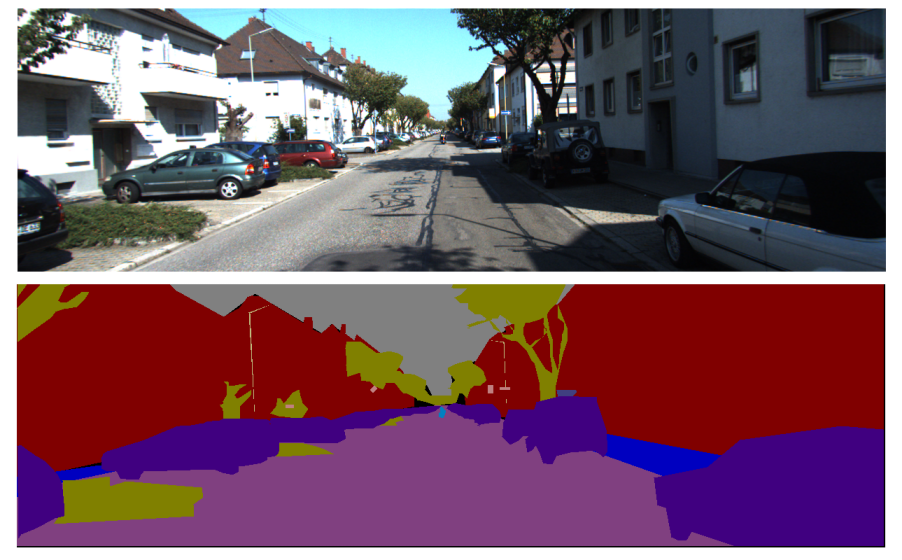
\includegraphics[width=\textwidth]{imgs/kitti-example.png}
\caption{Primjer slike i oznake KITTI skupa podataka}
\label{fig:kitti_example}
\end{figure}

\chapter{Implementacija}

U okviru ovog rada implementirana je radna okolina\footnote{\emph{https://github.com/iborko/theano-conv-semantic}} \engl{framework} za semantičku segmentaciju. U pozadini se koristi alat \textit{Theano}\footnote{Theano, \emph{http://deeplearning.net/software/theano/}} \cite{Theano-2012} \cite{Theano-2010} koji služi za definiranje, optimiranje i prevođenje simboličkih izraza u C++ ili CUDA programski kod.

Neke od prednosti korištenja alata \textit{Theano} su:
\begin{itemize}
	\item omogućuje paraleno korištenje CPU-a i GPU-a što ima za posljedicu da se algoritmi i programi mogu pisati i analizirati na nekom lošijem računalu, dok se ne utvrdi da rade dobro, a kasnije pokretati na računalima s moćnim grafičkim karticama bez kojih je ozbiljniji rad s velikim skupovima podataka i dubokim mrežama praktički nezamisliv
    \item optimiranje simboličkih izraza, što znači da se nijedan izraz neće računati više od jednom
    \item aritmetička pojednostavljenja, na primjer: $(x \cdot y)/x$ postaje $y$
    \item ugrađeno računanje gradijenata
    \item ugrađene metode za poboljšanje numeričke stabilnosti određenih matematičkih izraza
    \item ugrađen konvolucijski operator $\left( * \right)$
\end{itemize}
Mana korištenja \textit{Theana} upravo je to što on nije programski jezik, već se u programskom jeziku \textit{Python} pišu izrazi za \textit{Theano}. Za takvo pisanje izraza je potreban malo drugačiji način razmišljanja koji zahtjeva privikavanje.

Iako su neki alati, poput \textit{Caffe-a} i \textit{PyLearna-a}, jednostavniji za korištenje, mnogo je teže nadograđivati funkcionalnosti jer to iziskuje pisanje C++ i CUDA koda koji mora biti kompatibilan s već napisanim kodom, dok se u \textit{Theanu} samo definira simbolički izraz za novu funkcionalnost. U trenutku početka izrade ovog rada nisu postojali alati specijalizirani za semantičku segmentaciju, a eventualna proširenja postojećih alata (namijenjenih klasifikaciji) bila su u razvoju.

Parametri razvijene radne okoline poput arhitekture mreže, stope učenja, načina pretprocesiranja, vrste algoritma gradijentne optimizacije, i slično, definiraju se u konfiguracijskoj datoteci u JSON formatu koja se predaje kao argument skriptama za generiranje ulaza (pretprocesiranje) i učenje:
\begin{lstlisting}[language=bash]
    python generate.py network.conf
    python train.py network.conf
\end{lstlisting}
gdje je \texttt{network.conf} konfiguracijska datoteka u JSON formatu. Primjer datoteke je prikazan u dodatku \ref{chap:konfiguracijska datoteka}. JSON format je odabran jer se bazira na samo dvije strukture podataka: rječniku i listi, što su ujedno dvije glavne strukture koje koristi \textit{Python}. Preslikavanje JSON datoteke u \textit{Python} je zato vrlo jednostavno i implementirano u standardnim knjižnicama jezika \textit{Python}.

\section{Podatci}
Svaki skup podataka semantički segmentiranih slika koji se koristi mora imati svoju skriptu za učitavanje u mapi \texttt{dataset}. Tamo već postoje skripte \texttt{loader\_iccv.py} i \texttt{loader\_kitti.py} za učitavanje pripadnih datasetova. Svaka \texttt{loader\_*.py} skripta mora imati \texttt{load\_dataset(path)} funkciju koja vraća listu (ili iterator) \texttt{Sample} objekata. Razred \texttt{Sample} je definiran u \texttt{dataset/sample.py} datoteci i sadrži: naziv primjera, ulaznu sliku i segmentiranu sliku. Ulazne slike su u obliku \emph{numpy}\footnote{\textit{numpy}, ekstenzija jezika \textit{Python} koja dodaje podršku za višedimenzionalne brojevne nizove i podržava razne matematičke operacije nad njima, http://www.numpy.org} tenzora s 3 dimenzije: visina, širina i broj kanala, a izlazne slike su u obliku \emph{numpy} matrica gdje je element matrice oznaka (redni broj) pripadnog piksela.

\section{Pretprocesiranje}
Pomoću konfiguracijske datoteke moguće je definirati niz funkcija koja se koriste tijekom pretprocesiranja. Neki od primjera funkcija:
\begin{description}
  \item[yuv] pretvara RGB kanale u YUV kanale
  \item[int\_to\_float] pretvara intenzitete iz raspona od 0 do 255 (cijeli brojevi) u raspon 0 do 1 (decimalni brojevi)
  \item[normalize] normalizira sliku tako da svaki kanal ima srednju vrijednost intenziteta 0 i standardnu devijaciju 1
  \item[normalize\_block] normalizira sliku tako da svaki blok od $15 \cdot 15$ piksela svakog kanala ima srednju vrijednost intenziteta 0 i standardnu devijaciju 1
\end{description}


\section{Arhitektura mreže}
\label{chap:net_architecture}

Konvolucijska mreža korištena u radu je napravljena po uzoru na mrežu iz rada \cite{farabet_pami}. Mreža se može podijeliti u dvije logičke cjeline: detektor značajki i klasifikator. Detektor značajki sastoji se od konvolucijskih slojeva i slojeva sažimanja, a klasifikator se sastoji od potpuno povezanog sloja i multinomijalne regresije (višeslojne regresije za više razreda).

Sama mreža se trenira u dvije faze: tijekom prve faze se trenira samo detektor značajki, a tijekom druge faze samo klasifikacijski dio. U praksi to znači da se prvo na detektor značajki spoji samo multinomijalna regresija i trenira se takav sustav. Nakon toga se, u drugoj fazi, na detektor značajki spoji potpuno povezani sloj s \emph{dropout} slojem i slojem multinomijalne regresije i uče se samo njihove težine.

Detektor značajki sastoji se od tri paralelne razine. Svaka razina prima sliku drugačije veličine: prva razina prima originalnu sliku, druga razina prima sliku poduzorkovanu na pola dok treća prima sliku poduzorkovanu na četvrtinu originalne veličine. Svaka razina se sastoji od više slojeva: prvi konvolucijski sloj, sloj sažimanja, drugi konvolucijski sloj, sloj sažimanja, treći konvolucijski sloj. Izlaz svakog konvolucijskog sloja propušta se kroz \textit{lReLU} aktivacijsku funkciju definiranu formulom:
\begin{equation}
  lReLU( x ) = \max(x,\ \frac{1}{5} x)
\end{equation}

Ukupno je to devet konvolucijskih slojeva. No, slojevi na istim pozicijama u svih razinama dijele konvolucijske filtere: prvi konvolucijski sloj prve razine dijeli filtere s prvim konvolucijskim slojem druge i treće razine, itd. Time se uvelike smanjuje složenost modela (broj parametara), no glavna ideja takve arhitekture je otpornost na drugačije veličine objekata. Ako se neki filter prvog konvolucijskog sloja koristi za, na primjer, detekciju kotača na automobilu, onda on prepoznaje kotač određene veličine. No, što ako je kotač veći? Ovakvom arhitekturom je moguće prepoznati i veći kotač jer će druga razina primiti smanjenu sliku, a time i smanjeni kotač, čime on može biti detektiran istim filterom.

Budući da svaka razina ima ulaz drugačije veličine, razlikuju se i izlazi. Izlaz druge razine je upola manji nego izlaz prve razine, a izlaz treće razine četiri puta manji. Dobivene mape značajki su zatim ulaz u klasifikator. Ako zadnji konvolucijski sloj daje $k$ mapa značajki, ukupno u klasifiktor onda ulazi $3 \cdot k$ mapa značajki. Budući da se klasificira svaki piksel mape značajki, mape značajki svake razine moraju biti istih dimenzija. Ulaz se onda može prikazati kao:
\begin{equation}
	\boldsymbol{X} = [\boldsymbol{FM}_1, up(\boldsymbol{FM}_2, 2), up(\boldsymbol{FM}_3, 4)].flatten()
\end{equation}
gdje je $\boldsymbol{X}$ ulaz u klasifikator, $\boldsymbol{FM}_i$ je izlaz iz $i$-te razine detektora značajki (mapa značajki), $up(\boldsymbol{FM}, n)$ je funkcija naduzorkovanja koja mapu značajki $\boldsymbol{FM}$ s dimenzija $(x, y)$ transformira u dimenzije $(x \cdot n, y\cdot n)$ a $.flatten()$ je funkcija koja tenzor dimenzija $(x, y, k)$ pretvara u matricu dimenzija $(x \cdot y, k)$. Takva matrica predstavlja značajke svakog od $x \cdot y$ piksela.

Opisana mreža na ulaz prima cijelu sliku za segmentaciju. Detektori značajki tada generiraju mape značajki i provodi se klasifikacija svakog ''piksela'' te mape značajki. To znači da za jednu sliku na ulazu klasifikator provodi $x \cdot y$ klasifikacija piksela odjednom, ako su $x$ i $y$ dimenzije mape značajki.

Definirajmo i pojmove iteracija i epohe. \textbf{Iteracija} se sastoji od jedne unaprijedne propagacija i jedne unazadne propagacija, što znači jedno podešavanje gradijenata. Jednom se iteracijom može obraditi jedna slika, ili skup od više slike \engl{mini batch}. \textbf{Epoha} je jedno iteriranje kroz cijeli skup za učenje, kad svi primjeri prođu jednom kroz mrežu.

Realizirana arhitektura modificira skup za učenje nakon svake epohe koristeći slučajne transformacije opisane u poglavlju \ref{chap:dataset_perturbations}. Koristi se skaliranje slike za faktor u rasponu $[1.0, 1.1]$, rotacija za kut u rasponu $[-10, 10]$ stupnjeva, smik u rasponu $[-5, 5]$ stupnjeva i translacija u rasponu $[-20, 20]$ piksela.


\section{Postprocesiranje}

Semantičke oznake koje generira implementirana radna okolina su šumovite i ne prate dobro konture objekata i regija na slici. Zato se često koriste metode zaglađivanja tih predikcija: superpikseli ili grafički modeli. Superpiksel jednostavno označava nakupinu piksela. Postoje razne metode pod nazivom superpikseli koje čine takva grupiranja.

U ovom radu korištena je metoda iz rada \cite{Felzenszwalb04}, koja grupira piksele, ovisno o sličnosti u njihovom susjedstvu. Preuzet je autorov javno objavljen\footnote{\textit{http://ttic.uchicago.edu/~xren/research/superpixel/}} kod u programskoj jeziku C i napisan je prilagodnik u \textit{Cythonu}\footnote{Cython, prošitenje Python jezika statičkim tipovima, s proširenjima za jezik C} koji omogućuje korištenje C i C++ koda kao \textit{python} modula. Za svaku nakupinu piksela, odredi se oznaka koja je nazastupljenija, a zatim se sve oznake nakupine promijene u tu oznaku.

\begin{figure}[tb]
\centering
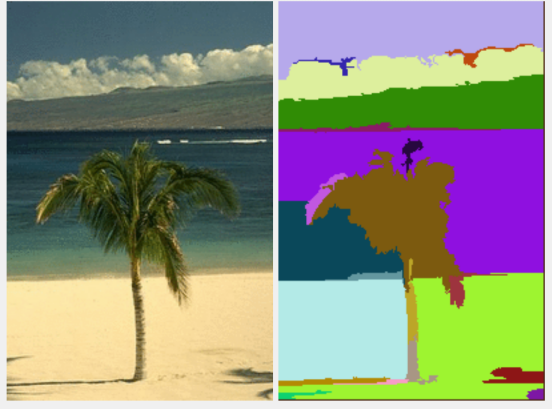
\includegraphics[width=340px]{imgs/superpixel.png}
\caption{Segmentacija superpikselima}
\end{figure}

\section{Stopa učenja}

Vrsta gradijentne metode koja se koristi (i njezini parametri) definiraju se u konfiguracijskoj datoteci, u dijelu \texttt{optimization} i \texttt{optimization-params}. Svaka metoda koristi stopu učenja kao jedan od parametara. U implementaciji ovoga rada se koristi postupak dinamčkog smanjivanja stope učenja: početna stopa učenja se prepolovi svaki put kada se poboljšanje funkcije troška na skupu za učenje \engl{train set} nije desilo zadnjih \texttt{no-improvement-epochs} epoha. Smanjivanje se provodi dok je stupa učenja veća od \texttt{min-learning-rate}. \texttt{no-improvement-epochs} i \texttt{min-learning-rate} su parametri definirani u konfiguracijskoj datoteci.

\section{Uvjeti zaustavljanja}
Učenje mreže treba provoditi sve dok ima poboljšanja na skupu za provjeru, ali opet ne predugo kako se model ne bi prenaučio. U sklopu ovog rada implementirana je metoda koja prekida učenje ako nema poboljšanja funkcije troška na skupu za provjeru \engl{validation set} zadnjih $p$ epoha. $p$ se na početku postavlja na vrijednost od 20 epoha. Svaki put kada se desi poboljšanje, $p$ se promijeni:
\begin{equation}
  p := \max \left( p, 10 + 1.1 \cdot epoch \right)
\end{equation}
gdje je $epoch$ trenutna epoha učenja. Time se postiže da učenje traje barem 20 epoha, a nakon svakog poboljašanja se $p$ postavi na vrijednost veću za 10 epoha i 10\% epoha od trenutne epohe.

Uzmimo za primjer da je trenutna epoha 50 i desi se poboljšanje. Vrijednost $p$ će tada postati $50 \cdot 1.1 + 10 = 65$. To znači da će se učenje provoditi barem do 65. epohe. Svako poboljašanje u međuvremenu će opet povećati $p$. Što je postupak učenja više napredovao (podrazumijeva i manju stopu učenja), daje mu se više vremena za postizanje boljeg rezultata.


\chapter{Rezultati}

Konvolucijska neuronska mreža implementirana u ovom radu je evaluirana na nekoliko poznatih skupova podataka. Rezultati su uspoređeni s rezultatima ostalih autora i napravljena je usporedba kako određene metode utječu na rezultate evaluacije.

Mreža je trenirana na računalu s Intel i7-4790 procesorom s 8 virtualnih jezgri, 16 GB RAM-a i grafičkom karticom nVidia GTX 970. Računalo s grafičkom karticom omogućilo je pokretanje Theana u GPU načinu rada, čime se sav kod prevodio u CUDA kod, što je ubrzalo izvođenje za faktor veličine 100 (naspram izvođenja na i5 procesoru).

\section{Mjere}

Najjednostavnija mjera kod klasifikacije je točnost \engl{accuracy}, odnosno omjer broja točno klasificiranih primjera naspram ukupnog broja primjera. Kad se govori o semantičkoj klasifikaciji, govorimo o \textbf{točnosti piksela} \engl{pixel accuracy}, odnosno broju točno označenih piksela naspram ukupnog broja piksela.

No, budući da su kod semantičke segmentacija klase često neravnomjerno zastupljene, događa se da model skroz zanemaruje rijetko zastupljene razrede, čime će postići visoku točnost klasifikacije piksela. No mi to želimo uravnotežiti, tj želimo postići da model prepoznate i rijetko zastupljene znakove koji su često važni (primjer su prometni znakovi).

Tako se dolazi do druge mjere, \textbf{srednje točnosti razreda} \engl{class accuracy, mean class accuracy}. Ta mjera se definira kao prosjek točnosti svih razreda. Ako je $accuracy(\mathcal{D}, c)$ funkcija koja vraća točnost klasifikacije razreda $c$ na skupu primjera $\mathcal{D}$ i $C$ skup svih razreda, onda srednju točnost razreda možemo definirati kao:
\begin{equation}
  class\_accuracy \left( \mathcal{D} \right) = \frac{1}{\abs{C}} \sum_{c=1}^{\abs{C}} accuracy(\mathcal{D}, c)
\end{equation}

\textbf{IOU}\engl{intersection over union} je isto mjera često korištena kod semantičke segmentacije. Ona se definira kao:
\begin{equation}
  IOU \left( \mathcal{D} \right) = \frac{1}{\abs{C}} \sum_{c=1}^{\abs{C}} \frac{\abs{\boldsymbol{y}_p(c) \cap \boldsymbol{y}_t(c)}}{\abs{\boldsymbol{y}_p(c) \cup \boldsymbol{y}_t(c)}}
\end{equation}
gdje je $C$ skup svih razreda, $\boldsymbol{y}_t$ je skup oznaka za učenje, a $\boldsymbol{y}_p$ je predviđeni skup oznaka.

\section{Stanford Background Dataset}

Na \textit{Stanford Background} skupu za učenje korištena je arhitektura mreže opisana u poglavlju \ref{chap:net_architecture}. Slike su prije ulaza u mrežu pretvorene iz RGB spektra u YUV spektar, zatim su napravljene 3 razine Laplaceove piramide (jedna razina piramide za jednu razinu mreže) i vrijednosti svakog kanala su normalizirane na raspon $\left[ 0, 1 \right]$.

Prvi konvolucijski sloj transformira 3 ulazna kanala (YUV) u 16 izlaznih mapa značajki: 10 mapa značajki je spojeno isključivo na Y kanal, a preostalih 6 na U i V kanale. Drugi konvolucijski sloj transformira 16 mapa u 64 mape značajki, a treći te 64 mape u konačnih 256 mapa. Budući da postoje 3 razine, svaka daje 256 mapa značajki, što znači da je svaki piksel opisan sa $256 \cdot 3 = 768$ značajki. Svaka razina ima dva sloja sažimanja, tako da od ulazne slike dimenzija 320 x 240 na izlazu zadnjeg konvolucijskog sloja prve razine dobijemu mape značajki dimenzija 80 x 60, odnosno 40 x 30 i 20 x 15 za drugu i treću razinu. Izlazi druge i treće razine su naduzorkuju da bi se dobio 768 mapa značajki dimenzija 80 x 60. Semantičke oznake dobivene mrežom se onda moraju povećati do prave dimenzionalnosti označene slike iz skupa za učenje i usporediti.

U drugoj fazi učenja se dodaje potpuno povezani sloj sa 1000 neurona, \textit{dropout} sloj (sa $p=0.5$) i sloj multinomijalne regresije sa 9 izlaza, što rezultate obično poboljša za jedan do dva posto (naspram multinomijalne regresije izravno spojene na detektor značajki). Prosječno vrijeme učenja mreže je oko 4 sata. Od gradijentnih metoda koristi se Rmsprop sa početnom stopom učenja $2 \cdot 10^{-4}$, a u prvoj fazi koristi se i $L_2$ regularizacija s faktorom $10^{-5}$.

Mreža opisana u ovom radu u jednom prolazu segmentira cijelu sliku. Sa stajališta brzine i memorije to je odlično, ali problem predstavljaju nebalansirani skupovi podatka. U takvoj arhitekturi nije moguće balasirati skupove podataka poduzorkovanjem ili naduzorkovanjem tako da predstavnika svih razreda bude podjenako. Zato je mreža je evaluirana s dvije različite funkcije troška: s običnom funkcijom negativne log izglednosti i Bayesovom funkcijom log izglednosti\cite{daylac} koja povećava trošak (a time i iznos gradijenata) slabo zastupljenih razreda. Bayesova negativna log izglednost je definirana formulom:
\begin{equation}
  bayesian\_nll = - \frac{1}{N} \sum_{i=1}^{N} \ln P(Y_i = c_i) \cdot \frac{1}{P_apr(c_i)}
\end{equation}
gdje je $P(Y = c_i)$ vjerojatnost da $i$-ti primjer pripada razredu $c_i$, $c_i$ je razred u koji $i$-ti primjer pripada, $P_apr(c_i)$ je apriorna vjerojatnost $i$-tog razreda.

\begin{table}
\centering

\begin{adjustbox}{center}
\begin{tabular}{l r r r}
  Metoda & Točnost(\%) & Točnost razreda(\%) & Brzina (sec) \\
    \multicolumn{2}{c}{Funkcija troška} & & \\[0.6em] \hline

  Konv. mreža s 3 razine & 75.7 & 59.3 & 0.05 \\
    \multicolumn{2}{c}{negativna log izglednost} & & \\ \hline
  Konv. mreža s 3 razine + \textit{superpixels} & 76.1 & 59.7 & 0.11 \\
    \multicolumn{2}{c}{negativna log izglednost} & & \\ \hline
  Konv. mreža s 3 razine & 71.4 & 64.8 & 0.05 \\
    \multicolumn{2}{c}{Bayesova log izglednost} & & \\ \hline
  Konv. mreža s 3 razine + \textit{superpixels} & 74.2 & 68.1 & 0.11 \\
    \multicolumn{2}{c}{Bayesova log izglednost} & & \\ \hline \hline
    
  Farabet et al.\cite{farabet_pami} 2013 & 78.8 & 72.4 & 0.6 \\ \hline
  Farabet et al.\cite{farabet_pami} 2013 + \textit{superpixels} & 80.4 & 74.6 & 0.7 \\ \hline
  Lempitzky et al.\cite{lempitsky11} 2011 & 81.9 & 72.4 & >60 \\ \hline
  Munoz et al.\cite{munoz10} 2010 & 76.9 & 66.2 & 12
\end{tabular}
\end{adjustbox}

\caption{Rezultati na Stanford Background skupu podataka}
\end{table}

Slučajno je odabrano je 15\% slika koje se koriste kao skup za testiranje, na kojima su dobiveni prikazani rezultati. Tijekom učenja 10\% slika je izuzeto iz procesa učenja i korišteno kao skup za provjeru  kako bi se odredio trenutak zaustavljanja.

Mreža je testirana koristeći 5 preklopa na skupu podataka \engl{5-folded cross validation}, a 10\% slika je izuzeto iz procesa učenja i korišteno kao skup za provjeru\engl{validation set} te kako bi se odredio trenutak zaustavljanja.

Slika \ref{fig:iccv_train} prikazuje vrijednost funkcije troška i pogreške na skupu za provjeru tijekom učenja. Kao funkcija troška korištena je funkcija negativne log izglednosti. Nagli skok pred kraj učenja je trenutak početka druge faze učenja.

\begin{figure}[htb]
  \centering
  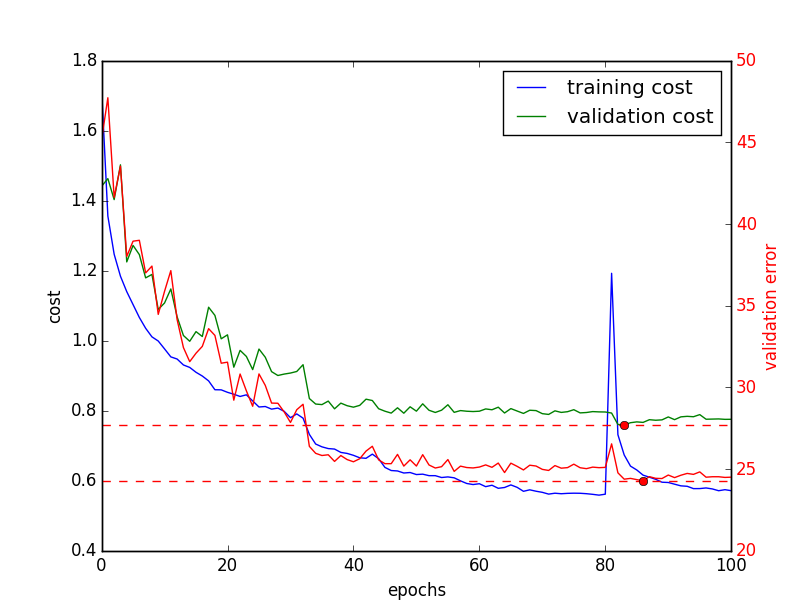
\includegraphics[width=\textwidth]{imgs/cost-iccv.png}
  \caption{Funkcija troška i greška tijekom učenja na Stanford Background podacima}
  \label{fig:iccv_train}
\end{figure}

\section{KITTI}

I na ovom skupu podataka korištena je arhitektura opisana u poglavlju \ref{chap:net_architecture}, no ovoga puta ideja je bila isprobati dataset koji osim RGB slike ima i dubinsku komponentu (dubinu za svaki piksel slike). Dubinska komponenta je dobivena stereoskopskom rekonstrukcijom (slike za rekonstrukciju su javno objavljene). Sve slike su veličine 1241 x 386 piksela, ali su zbog memorijskih zahtjeva smanjene na 620 x 192 piksela. Ulaz u mrežu sastojao se od slike s 4 kanala: 3 YUV kanala i dubinska komponenta D. Napravljena je Laplace-ova piramida od 3 razine koristeći YUV komponente, dok je dubinska mapa samo smanjena na pola, odnosno četvrtinu i dodana razinama Laplaceove piramide kao četvrti kanal.

Isprobana je varijanta mreže gdje se koriste samo RGB slike (transformirane u YUV i Laplaceovu piramidu) i varijanta gdje se koristi i dubinska mapa. U mreži koja koristi samo RGB kanale prvi konvolucijski sloj ima 16 filtera (10 spojeno na Y komponentu, 6 na UV komponente), drugi ima 64 filtera, a treći ima 256 filtera.
Mreža koja koristi i dubinsku informaciju ima jednak raspored filtera, osim što su u prvom sloju svi filteri spojeni na svaki od četiri RGBD kanala.

I na ovom skupu za učenje korištena je metoda učenja u dvije faze. U drugoj fazi dodaje se potpuno povezani sloj od 1000 neurona i \textit{dropout} sloj. Tijekom prve faze koristi se i $L_2$ regularizacija s faktorom $10^{-5}$.

\begin{table}
\centering

\begin{adjustbox}{center}
\begin{tabular}{l r r r}
  Metoda & Točnost(\%) & Točnost razreda(\%) & Brzina (sec) \\
    \multicolumn{2}{c}{Funkcija troška} & & \\[0.6em] \hline

  Konv. mreža s 3 razine (RGB) & 73.6 & 42.4 & 0.05 \\
    \multicolumn{2}{c}{negativna log izglednost} & & \\ \hline
  Konv. mreža s 3 razine (RGB) + \textit{superpixels} & 75.1 & 43.1 & 0.11 \\
    \multicolumn{2}{c}{negativna log izglednost} & & \\ \hline
  Konv. mreža s 3 razine (RGB) & 69.8 & 55.3 & 0.05 \\
    \multicolumn{2}{c}{Bayesova log izglednost} & & \\ \hline
  Konv. mreža s 3 razine (RGBD) & 78.5 & 45.8 & 0.05 \\
    \multicolumn{2}{c}{negativna log izglednost} & & \\ \hline
  Konv. mreža s 3 razine (RGBD) + \textit{superpixels} & 79.1 & 46.1 & 0.11 \\
    \multicolumn{2}{c}{negativna log izglednost} & & \\ \hline \hline
    
  Ros et al.\cite{ros:2015} 2015 & 81.1 & 58.0 & 0.46
\end{tabular}
\end{adjustbox}

\caption{Rezultati na KITTI skupu podataka}
\end{table}

Slika \ref{fig:kitti_train} prikazuje vrijednost funkcije troška na skupovima za učenje i provjeru te grešku na skupu za provjeru tijekom učenja. Korištena je verzija mreže koja uzima u obzir i dubinske podatke. Vidljivo je da je učenje trajalo sedamdesetak epoha. Nagli skok pred kraj učenja je završetak prve faze učenja i početak druge faze.

\begin{figure}[htb]
  \centering
  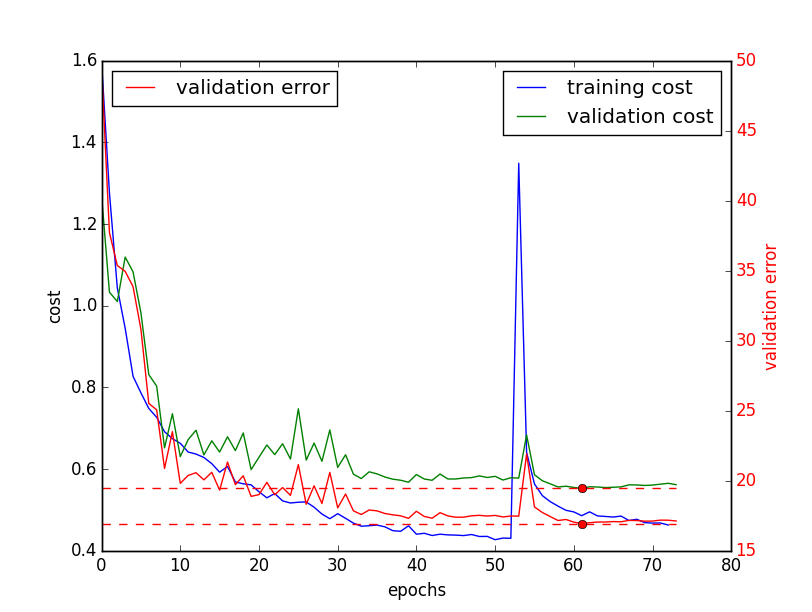
\includegraphics[width=\textwidth]{imgs/cost-kitti-rgbd.png}
  \caption{Funkcija troška i greška tijekom učenja na KITTI podacima, za RGBD verziju mreže mrežu}
  \label{fig:kitti_train}
\end{figure}

\chapter{Zaključak}

Područje dubokih neuronskih mreža nedavno se počelo ubrzano razvijati, a u mnogim područjima računalnog vida već postiže odlične rezultate. U ovom radu opisane su neuronske mreže, s naglaskom na konvolucijske neuronske mreže, metode učenja neuronskih mreža te mnogi detalji oko njihovog korištenja.

U sklopu ovog rada implementiran je cjelokupni sustav za semantičku segmentaciju korištenjem konvolucijskih neuronskih mreža. Sustav je realiziran korištenjem radne okoline \textit{Theano} koja omogućuju pokretanje koda na grafičkim karticama s podrškom za CUDA jezik. Izgrađeni sustav se sastoji od slojeva neuronskih mreža poput konvolucijskih slojeva, slojeva sažimanja, potpuno povezanog sloja, multinomijalne regresije i slično, koji se mogu kombinirati u razne arhitekture.

Arhitektura korištena u ovoj implementaciji napravljena je po uzoru na arhitekturu koju su predložili Farabet et al.\cite{farabet_pami}. Osim same mreže napisane su razne gradijentne metode poput stohastičkog gradijentnog spusta i \textit{Rmsprop}-a, mnoge aktivacijske funkcije, skripte za pretprocesiranje slika i postprocesiranje rezultata.

Arhitektura je prvo testirana na Stanford Background skupu podatka gdje su postignuti rezultati usporedivi s onima u drugim radovima. Taj sustav je radio samo s RGB slikama na ulazu. Nakon toga je sustav proširen tako da može primati i RGB-D slike i evaluiran na KITTI skupu podataka za semantičku segmentaciju gdje je isto postigao relevantne rezultate.

Daljnjim razvojem područja konvolucijskih neuronskih mreža, ali i samog sklopovlja poput specijaliziranih grafičkih kartica semantička segmentacija pomoću konvolucijskih mreža trebala bi davati sve bolje rezultate.

\bibliography{literatura}
\bibliographystyle{fer}

\appendix

\chapter{Detalji implementacije}
\section{Primjer koda u Theanu}

\begin{lstlisting}[language=python]
>>> import theano
>>> a = theano.tensor.vector()
>>> a
  <TensorType(float32, vector)>
>>> out = a + a ** 10
>>> out
  Elemwise{add,no_inplace}.0
>>> f = theano.function([a], out)   # compile
>>> print f([0, 1, 2])
  array([0, 2, 1026])
\end{lstlisting}
Naveden je primjer koda u \textit{Theanu} kako bi se lakše pojmio način rada s njime. Prvo se definira simbolička varijabla \texttt{a} koja predstavlja vektor, što znači da će \textit{Theano} tijekom izvođenja očekivati da njezina vrijednost bude vektor brojeva. Ovisno o vrsti simboličke varijable, \textit{Theano} koristi drugačije vrste operatora i drugačije optimira kod. Osim toga, \textit{Theano} očekuje da će brojevi u vektoru biti u formatu \textit{float32}. Kod kreiranja simboličke varijable, moguće je odabrati i neki drugi tip (\textit{int8}, \textit{int32}, \textit{float64}, ...). Varijabla \texttt{out} definira se kao simbolički izraz koji sadrži operator +. \textit{Python} to vidi kao \textit{Theano} \textit{Elemwise} objekt. Na kraju se stvara funkcija \texttt{f} čiji je ulaz simbolička varijabla \texttt{a}, a izlaz je simbolička varijabla \texttt{out} (koja ovisi o \texttt{a}).

Izvođenje naredbe koja stvara funkciju obično traje nekoliko sekundi. Razlog tome je što \textit{Theano} u tom trenutku krene optimirati simboličko stablo izvođenja funkcije, zatim odabere vrstu izvršnog koda (C++ ili CUDA) i na kraju prevodi graf u izvršni kod. Kad se nakon toga pozove funkcija \texttt{f}, ta funkcija se zapravo izvršava u tom prevednom i optimiranom C++ ili CUDA kodu.


\section{Konfiguracijska datoteka}
\label{chap:konfiguracijska datoteka}

Primjer konfiguracijske datoteke za učenje mreže, u JSON formatu.
\begin{lstlisting}[language=json]
{
    "evaluation": {
        "batch-size": 4
    },
    "network": {
        "layers": [16, 64, 256, 1000],
        "loss": "negative_log_likelihood",
        "builder-name": "build_multiscale",
        "seed": 23451
    },
    "training": {
        "optimization": "rms",
        "optimization-params": {
            "learning-rate": 0.0002,
            "momentum": 0.9
        },
        "epochs": -1,
        "learning-rate-decrease-params": {
            "no-improvement-epochs": 4,
            "min-learning-rate": 0.00001
        }
    },
    "training2": {
        "optimization": "rms",
        "optimization-params": {
            "learning-rate": 0.0001,
            "momentum": 0.9
        },
        "epochs": 130,
        "learning-rate-decrease-params": {
            "no-improvement-epochs": 3,
            "min-learning-rate": 0.00001
        }
    },
    "data": {
        "location": "data/kitti/theano_datasets/",
        "dont-care-classes": [0]
    }
}
\end{lstlisting}
\texttt{"tranining"} označava prvu fazu učenja (učenje generatora značajki), \texttt{"training2"} označava drugu fazu učenja (učenje klasifikatora). \texttt{"epochs": -1} označava da je broj epoha neograničen.

\chapter{Slike rezultata}
Prikazano je nekoliko primjera rada programa, na primjerima iz skupova za testiranje. Slika gore desno je originalna slika, slika gore desno je slika iz skupa za učenje označena semantičkim oznakama, slika dolje lijevo su oznake dobivene iz mreže, a dolje desno su oznake zaglađene \textit{superpixel} metodom.

\section{Stanford Background}
Primjeri su dobiveni mrežom koja je učena funkcijom negativne log izglednosti.

\begin{figure}[H]
  \centering
  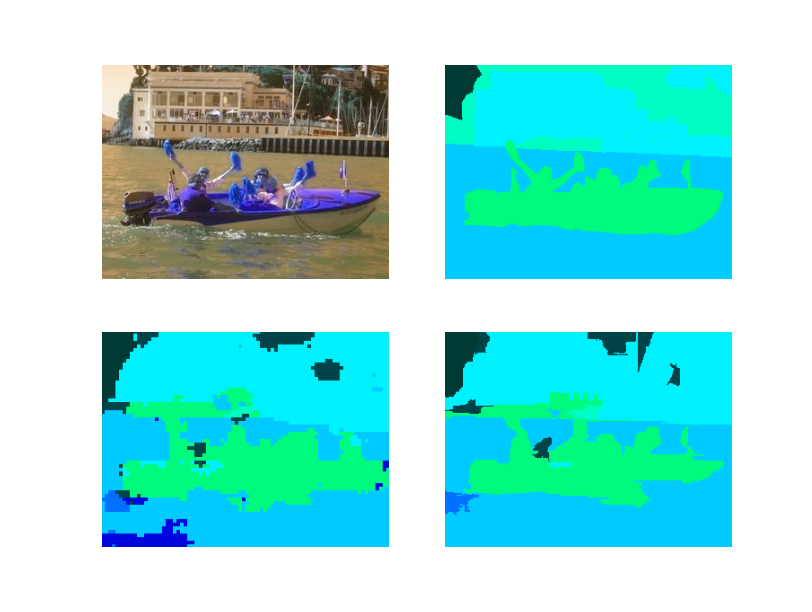
\includegraphics[width=\textwidth]{imgs/iccv-sampl2.png}
  \caption{Rezultati na Stanford Background skupu podataka}
\end{figure}

\begin{figure}[H]
  \centering
  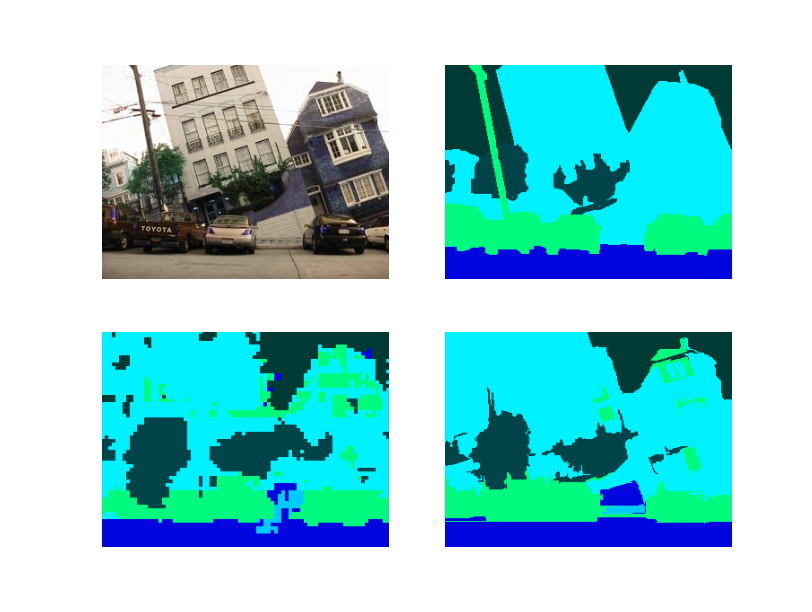
\includegraphics[width=\textwidth]{imgs/iccv-sampl3.png}
  \caption{Rezultati na Stanford Background skupu podataka}
\end{figure}

\section{KITTI}
Primjeri su dobiveni mrežom koja je učena na RGBD podacima, a kao funkcija troška korištena je funkcija negativne log izglednosti.

\begin{figure}[H]
  \centering
  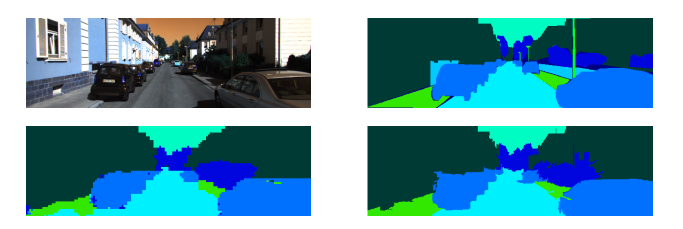
\includegraphics[width=\textwidth]{imgs/kitti3.png}
  \caption{Rezultati na KITTI skupu podataka}
\end{figure}

\begin{figure}[H]
  \centering
  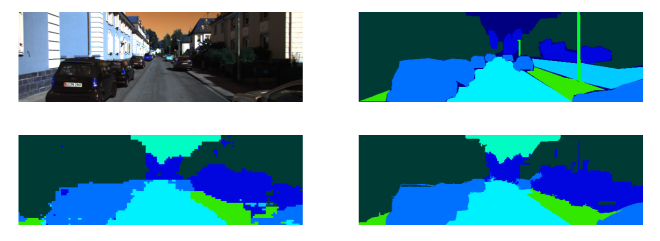
\includegraphics[width=\textwidth]{imgs/kitti4.png}
  \caption{Rezultati na KITTI skupu podataka}
\end{figure}

\newpage

\begin{sazetak}
U ovom radu opisane su duboke neuronske mreže, s posebnim naglaskom na konvolucijske neuronske mreže. Detaljno su obrađene metode i postupci koji se koriste kod učenja konvolucijskih neuronskih mreža. Implementirana je konvolucijska mreža za semantičku segmentaciju u Theano radnoj okolini i isprobana na dva skupa podataka: Stanford Background skupu podatka koji za ulaz ima RGB slike i na KITTI skupu podataka koji na ulazu ima RGB-D slike. Na kraju su prikazani dobiveni rezultati, s opisima i slikama.

\kljucnerijeci{računalni vid, neuronske mreže, konvolucijske mreže, duboko učenje, semantička segmentacija}
\end{sazetak}

% naslov na engleskom jeziku
\engtitle{Semantic segmentation of outdoor scenes using deep neural networks}
\begin{abstract}
This work describes deep neural networks, with emphasis on convolutional neural networks. Gradient methods and learning algorithms used for neural networks learning are shown. Convolutional network for semantic segmentation problems is built using Theano framework and it's performance is evaluated on two datasets: Stanford Background dataset, consisting of only RGB images and KITTI dataset, consisting of RGB-D images. Following that, numerical results are presented, together with descriptions and images.

\keywords{computer vision, neural networks, convolutional networks, deep learning, semantic segmentation}
\end{abstract}

\end{document}